\documentclass[12pt, twoside, openright]{report} % Fuente a 12pt, formato doble página y chapter a la derecha
\raggedbottom % No ajustar el contenido con un salto de página

% MÁRGENES: 2,5 cm sup. e inf.; 3 cm izdo. y dcho.
\usepackage[
a4paper,
vmargin=2.5cm,
hmargin=3cm
]{geometry}

% INTERLINEADO: Estrecho (6 ptos./interlineado 1,15) o Moderado (6 ptos./interlineado 1,5)
\renewcommand{\baselinestretch}{1.15}
\parskip=6pt

% DEFINICIÓN DE COLORES para portada y listados de código
\usepackage[table]{xcolor}
\definecolor{azulUC3M}{RGB}{0,0,102}
\definecolor{gray97}{gray}{.97}
\definecolor{gray75}{gray}{.75}
\definecolor{gray45}{gray}{.45}

% Soporte para GENERAR PDF/A
\usepackage{etoolbox}
\makeatletter
\@ifl@t@r\fmtversion{2021-06-01}%
 {\AddToHook{package/after/xmpincl}
   {\patchcmd\mcs@xmpincl@patchFile{\if\par}{\ifx\par}{}{\fail}}}{}
\makeatother
\usepackage[a-1b]{pdfx}

% ENLACES
\usepackage{hyperref}
\hypersetup{colorlinks=true,
  linkcolor=black, % enlaces a partes del documento (p.e. índice) en color negro
  urlcolor=blue} % enlaces a recursos fuera del documento en azul

% Añadir pdfs como partes del documento
\usepackage{pdfpages}

% Quitar la indentación de principio de los párrafos
\setlength{\parindent}{0em}

% EXPRESIONES MATEMÁTICAS
\usepackage{amsmath,amssymb,amsfonts,amsthm}

\usepackage{txfonts} 
\usepackage[T1]{fontenc}
\usepackage[utf8]{inputenc}

% Insertar gráficas y fotos
\usepackage{tikz}
\usepackage{pgfplots}

\usepackage[spanish, es-tabla]{babel} 
\usepackage[babel, spanish=spanish]{csquotes}
\AtBeginEnvironment{quote}{\small}

% diseño de PIE DE PÁGINA
\usepackage{fancyhdr}
\pagestyle{fancy}
\fancyhf{}
\renewcommand{\headrulewidth}{0pt}
\fancyfoot[LE,RO]{\thepage}
\fancypagestyle{plain}{\pagestyle{fancy}}

% DISEÑO DE LOS TÍTULOS de las partes del trabajo (capítulos y epígrafes o subcapítulos)
\usepackage{titlesec}
\usepackage{titletoc}
\titleformat{\chapter}[block]
{\large\bfseries\filcenter}
{\thechapter.}
{5pt}
{\MakeUppercase}
{}
\titlespacing{\chapter}{0pt}{0pt}{*3}
\titlecontents{chapter}
[0pt]                                               
{}
{\contentsmargin{0pt}\thecontentslabel.\enspace\uppercase}
{\contentsmargin{0pt}\uppercase}                        
{\titlerule*[.7pc]{.}\contentspage}                 

\titleformat{\section}
{\bfseries}
{\thesection.}
{5pt}
{}
\titlecontents{section}
[5pt]                                               
{}
{\contentsmargin{0pt}\thecontentslabel.\enspace}
{\contentsmargin{0pt}}
{\titlerule*[.7pc]{.}\contentspage}

\titleformat{\subsection}
{\normalsize\bfseries}
{\thesubsection.}
{5pt}
{}
\titlecontents{subsection}
[10pt]                                               
{}
{\contentsmargin{0pt}                          
  \thecontentslabel.\enspace}
{\contentsmargin{0pt}}                        
{\titlerule*[.7pc]{.}\contentspage}  

% DISEÑO DE TABLAS.
\usepackage{multirow} % permite combinar celdas 
\usepackage{caption} % para personalizar el título de tablas y figuras
\usepackage{floatrow} % utilizamos este paquete y sus macros \ttabbox y \ffigbox para alinear los nombres de tablas y figuras de acuerdo con el estilo definido. Para su uso ver archivo de ejemplo 
\usepackage{array} % con este paquete podemos definir en la siguiente línea un nuevo tipo de columna para tablas: ancho personalizado y contenido centrado
\newcolumntype{P}[1]{>{\centering\arraybackslash}p{#1}}
\DeclareCaptionFormat{upper}{#1#2\uppercase{#3}\par}

% Diseño de tabla para ingeniería
\captionsetup[table]{
  format=hang,
  name=Tabla,
  justification=centering,
  labelsep=colon,
  width=.75\linewidth,
  labelfont=small,
  font=small,
}

% DISEÑO DE FIGURAS.
\usepackage{graphicx}
\graphicspath{{img/}} %ruta a la carpeta de imágenes

% Diseño de figuras para ingeniería
\captionsetup[figure]{
  format=hang,
  name=Fig.,
  singlelinecheck=off,
  labelsep=colon,
  labelfont=small,
  font=small    
}

% NOTAS A PIE DE PÁGINA
\usepackage{chngcntr} % Para numeración continua de las notas al pie
\counterwithout{footnote}{chapter}

% LISTADOS DE CÓDIGO
% soporte y estilo para listados de código. Más información en https://es.wikibooks.org/wiki/Manual_de_LaTeX/Listados_de_código/Listados_con_listings
\usepackage{listings}

% definimos un estilo de listings
\lstdefinestyle{estilo}{ frame=Ltb,
  framerule=0pt,
  aboveskip=0.5cm,
  framextopmargin=3pt,
  framexbottommargin=3pt,
  framexleftmargin=0.4cm,
  framesep=0pt,
  rulesep=.4pt,
  backgroundcolor=\color{gray97},
  rulesepcolor=\color{black},
  %
  basicstyle=\ttfamily\footnotesize,
  keywordstyle=\bfseries,
  stringstyle=\ttfamily,
  showstringspaces = false,
  commentstyle=\color{gray45},     
  %
  numbers=left,
  numbersep=15pt,
  numberstyle=\tiny,
  numberfirstline = false,
  breaklines=true,
  xleftmargin=\parindent
}

\captionsetup[lstlisting]{font=small, labelsep=period}
% fijamos el estilo a utilizar 
\lstset{style=estilo}
\renewcommand{\lstlistingname}{\uppercase{Código}}

\pgfplotsset{compat=1.17} 
%-------------
% DOCUMENTO
%-------------

\begin{document}
\pagenumbering{roman} % Se utilizan cifras romanas en la numeración de las páginas previas al cuerpo del trabajo

%----------
% PORTADA
%---------- 
\begin{titlepage}
	\begin{sffamily}
		\color{azulUC3M}
		\begin{center}
			\begin{figure}[H] % incluimos el logotipo de la Universidad
				\makebox[\textwidth][c]{
\includegraphics[width=16cm]{Portada_Logo.png}}
			\end{figure}
			\vspace{2.5cm}
			\begin{Large}
				Grado en Ingeniería Informática\\
				2021-2022\\
				\vspace{2cm}
				\textsl{Apuntes}\\
				\bigskip
			\end{Large}
			{\Huge Algoritmos Genéticos y Evolutivos}\\
			\vspace*{0.5cm}
			\rule{10.5cm}{0.1mm}\\
			\vspace*{0.9cm}
			{\LARGE Jorge Rodríguez Fraile\footnote{\href{mailto:100405951@alumnos.uc3m.es}{Universidad: 100405951@alumnos.uc3m.es}  |  \href{mailto:jrf1616@gmail.com}{Personal: jrf1616@gmail.com}}}\\
			\vspace*{1cm}
		\end{center}
		\vfill
		\color{black}
		
\includegraphics[width=4.2cm]{img/creativecommons.png}\\
		Esta obra se encuentra sujeta a la licencia Creative Commons\\ \textbf{Reconocimiento - No Comercial - Sin Obra Derivada}
	\end{sffamily}
\end{titlepage}

%----------
% ÍNDICES
%---------- 

%--
% Índice general
%-
\tableofcontents
\thispagestyle{fancy}

%--
% Índice de figuras. Si no se incluyen, comenta las líneas siguientes
%-
\listoffigures
\thispagestyle{fancy}

%--
% Índice de tablas. Si no se incluyen, comenta las líneas siguientes
%-
\listoftables
\thispagestyle{fancy}

%----------
% TRABAJO
%---------- 

\pagenumbering{arabic} % numeración con números arábigos para el resto de la publicación  


%----------
% COMENZAR A ESCRIBIR AQUI
%---------- 

\chapter{Información}

\section{Profesores}
\begin{quote}
	Magistral: Pedro Isasi, pedro.isasi@uc3m.es, 2.1.B13.

	Práctica: Yago Sáez, yago.saez@uc3m.es, 2.1.C13

	Miércoles clases Práctica / Jueves clase Magistral.
\end{quote}

Las tutorías solicitarlas por correo electrónico, si no responden en 24-48 horas volver a enviar el mensaje, mejor insistir que perder el tiempo ante posible perdida.

Se utilizará portátil en las clases prácticas, traerlo para ir resolviendo los ejercicios de programación.

\section{Objetivos}
\begin{itemize}
	\item Trataremos de aprender métodos para replicar fundamentos biológicos, mediante programación evolutiva (Veremos estrategias históricas de la evolución, como Darwin o Mendel), para resolver problemas del campo de la Inteligencia Artificial.
	\item Se estudiarán y analizarán distintas técnicas de computación evolutiva que se basan en distintos paradigmas biológicos.
	\item Lo que buscamos es ser capaces de entender cómo funciona la inteligencia de las personas o animales para ver cómo se desarrollan los procesos y poder programarlos para que hagan una tarea o aprendan a hacerla.
\end{itemize}

Un ejemplo de aplicación consiste en desarrollo de antenas que se generan según distintas mediciones de señal de manera que se extenderá en aquellas direcciones que la maximicen, también evitando las interferencias. Este ejemplo se basa en las plantas, en la manera que tienen de ir buscando la luz para poder obtener energía y seguir creciendo.

También se emplean muchas basadas en insectos por su corta vida, que permiten observar la evolución de una manera más rápida.

Inteligencia artificial (no hay una única definición): Disciplina que consiste en diseñar programas que son capaces de resolver problemas de manera similar a un humano (razonamiento, aprendizaje o creatividad), pero sin haberles programado el proceso que les permite resolverlo, mediante una serie de casos base. De manera que dándole unos datos sea capaz de resolverlo, aprende a resolverlos.

\section{Evaluación continua}
\begin{itemize}
	\item 3 prácticas a lo largo del curso, que podrían ser 2 prácticas y una extensión de la primera.
	      \begin{itemize}
		      \item Consistirán en la entrega de una memoria siguiendo unos puntos dados y el código.
		      \item Individuales, excepto la última que es en equipo. 1 punto, 1.5 y 2.5 puntos
	      \end{itemize}
	\item 2 pruebas de evaluación, 2,5 puntos cada una.
	\item Examen final no obligatorio, si no se presenta a este la nota final será la de evaluación continua. Si te presentas se pondera la nota final tal que el 0.25 es evaluación continua y el 0.75 la nota del examen final.
	      \begin{itemize}
		      \item Sin hacer el examen final:
		            \begin{itemize}
			            \item 25 \% Parcial 1
			            \item 25 \% Parcial 2
			            \item 10 \% Práctica 1
			            \item 15 \% Práctica 2
			            \item 25 \% Práctica 3
		            \end{itemize}
		      \item Haciendo el examen final
		            \begin{itemize}
			            \item 6,3 \% Parcial 1
			            \item 6,3 \% Parcial 2
			            \item 2,5 \% Práctica 1
			            \item 3,8 \% Práctica 2
			            \item 6,3 \% Práctica 3
			            \item 75 \% Examen final
		            \end{itemize}
	      \end{itemize}
\end{itemize}

\chapter{Tema 1: Introducción a los algoritmos de Computación Evolutiva}
\section{Teoría genética}
Este tema nos permite entender de donde surge la intención de tratar de imitar los comportamientos biológicos y las teorías evolutivas que hay, en particular la evolución. Lo que trataremos es de acercarnos a como la biología es capaz de crear sistemas complejos.

\subsection{Los cuatro pilares de la evolución}
Dobzhansky (1973): “nothing in biology makes sense except in the light of evolution”.

\begin{itemize}
	\item \textbf{Población:} El conjunto de individuos.
	\item \textbf{Diversidad:} Es la variedad de individuos, que difieren en cualquier cosa, la naturaleza es la que se encarga de mantenerla y tiende a generar nueva diversidad. Las leyes de la naturaleza se dirigen a crearla.
	\item \textbf{Herencia:} Esencial para que se puedan transmitir la información entre individuos.
	\item \textbf{Selección:} Debe producirse la muerte de algunos individuos para que pueda seguir adelante la evolución, es fundamental.
\end{itemize}

\subsection{Selección Natural}
No es selección de los mejores, es un proceso estocástico, pueden sobrevivir individuos no tan buenos individualmente  pero si para el colectivo, porque mejoren la reproducción media.

La evolución no tiene un objetivo, no es un progreso, solo se adapta a las circunstancias y al medio. No necesariamente una generación en mejor que la anterior.

Actúa en el aquí y ahora, lo que es bueno en términos reproductivos aquí o ahora, puede no selo allí o después.

La vida no tiende a la complejidad, hay muchos más individuos simples que complejos.

En el mejor de los casos, la combinación de variedad, herencia y selección puede incrementar “hoy” la proporción de individuos cuyos padres disponían de características más propicias “ayer”.

\subsection{De donde viene la diversidad}
Viene de que la reproducción NO es perfecta, esto permite que haya ciertas imperfecciones (muy poco frecuentes) que les hagan más viables reproductivamente y se transmitan a sus descendientes, eso genera diversidad al haber pequeñas variaciones.

Aquellas características que no son ventajosas, pero tampoco afectan negativamente, son transmitidas también.

Es cuestión de estadística que se produzcan las variaciones, pero este proceso repetido innumerables veces, genera diversidad.

Permite al individuo “ensayar” nuevas funcionalidades, comportamientos, morfologías, nuevos nichos y propagar a generaciones futuras aquellos que mejor se adapten al entorno.

\subsection{Escala Evolutiva}
La vida se dio muy al comienzo de la vida de la Tierra, pero se han dado muchas grandes extinciones, una vez la vida se da la vida se va sabiendo abrir camino.

3.500 Ma para generar los primeros seres eucariotas pluricelulares.

Solo 500 Ma para generar el resto de los seres vivos (80 \% contra 20 \%).

Los organismos microscópicos, similares a aquello que evolucionaron tempranamente continúan siendo altamente exitosos y dominan la Tierra.

La mayor parte de las especias y la biomasa terrestre está constituida por procariotas.

\subsection{Primeros pasos}
\textbf{Moléculas replicantes → poblaciones de moléculas en compartimentos}. Favorece la cooperación entre replicantes, al estar dentro de una membrana común

\textbf{Replicadores independientes → cromosomas}. Los replicadores independientes se unen formando estructuras, cromosomas, que facilitan su supervivencia

\textbf{ARN como gen y enzima → ADN y proteína}. Se separa la información de los procesos enzimáticos

\textbf{Nace el código genético}. División del trabajo, aumento en la complejidad de lo producido

\subsection{Estromatolitos (-3500 Ma)}
Agrupaciones de células unicelulares en forma de colonias capaces de generar con energía solar un gas tóxico, O$_2$, de forma masiva.

A pesar de este gas tóxico la vida se adaptó para utilizar ese oxígeno.

\subsection{Célula eucariota (-3500 Ma a -1200 Ma)}
\textbf{Procariota → Eucariota}. Aparece un núcleo celular, donde está la información y orgánulos, esto ayuda a la supervivencia de la célula.

\subsection{Organismos pluricelulares (-540)}
Antes del cámbrico había organismos simples, paquetes de proteínas autoreplicantes tipo medusa o esponjas habitando el mar.

Se alimentaban de bacterias o filtrando el agua, no había plantas.

\subsection{El Cámbrico}
Aparecen cadenas tróficas complejas (animales que comen otros animales), todos los grandes filos (grandes divisiones de la naturaleza) de la naturaleza (50 en el cámbrico, antes solo había 1 y después 8 más, tras esto solo quedaban 20).

Cambió la faz de la tierra y conformaron la vida tal y como lo conocemos hoy.

Ocurrió en solo 5 millones de años.

\subsection{Periodo Cámbrico}
Antes del cámbrico organismos simples, paquetes de proteínas autoreplicantes tipo medusas o esponjas habitando el mar.

Se alimentaban de bacterias o filtrando el agua. No había plantas.

Aparecen cadenas tróficas complejas (animales comen otros animales).

De repente aparecen todos los grandes filos de la naturaleza, 50 en el cámbrico, solo 1 antes y 8 después (solo quedan 20).

Mares casi inertes en mares repletos de vida. Cambió la faz de la tierra y conformaron la vida tal y como la conocemos hoy.

Ocurrió en solo 5 millones de años.

Causas ambientales. La escasez de recursos dio lugar a una competencia ecológica que favoreció la coevolución “depredador- presa”.

Causas geológicas. La separación de los continentes permite la segregación de las poblaciones y la diversificación evolutiva.

Causas morfológicas. Aparición del mesodermo.

Permite la generación de estructuras de colágeno (piel, cartílago, músculos).

Esqueletos rígidos (huesos, conchas).

Proliferación de oxígeno. Los animales no están obligados a obtener el oxígeno por todo el cuerpo, sino por órganos específicos, dejando el resto para caparazones o exoesqueletos.

\subsection{Seres complejos}
\textbf{Clones asexuales → Poblaciones sexuales}, es el mecanismo que guía el proceso, permite generar más individuos y diversidad de una manera eficaz. Aparece el sexo.

\textbf{Protista → Animales, plantas y hongos}. Aparece la diferenciación celular, todas las células tienen todo el material genético. Cada tipo de célula tiene activa una pequeña parte de su material genético. Empiezan a aparecer organismos.

\textbf{Individuos solitarios → Colonias}, conjunto de organismos que funcionan como uno. Organismos sociales.

\subsection{Últimos pasos}
-500 Ma plantas y hongos colonizan la tierra.

Poco después aparecieron artrópodos y otros animales

-300 Ma aparecen los anfibios.

Seguidos por los primeros amniotas (reproducción ovípara en medio seco terrestre)

-200 Ma Mamíferos.

-100 Ma Aves.

-2 Ma Hombre. Algo peculiar de los humanos y simios es que son consciente de su propia existencia a diferencia de otros animales.

\subsection{Las leyes de Mendel}
Hizo experimentos con guisantes entre 1857 y 1868. Publico su primer artículo en 1866.

Se fijó en dos características, la altura de la planta y la rugosidad del guisante.

Mendel cruzó artificialmente plantas altas con bajas, y siempre se producían plantas altas.

Después cruzó las plantas resultantes y obtuvo unas proporciones de 3 a 1.

Elaboró una teoría corpuscularia de la herencia, que decía que la herencia está en alguna parte del individuo codificada.

Envió los resultados a un científico famoso, Nageli, pero pasó desapercibido.

50 años después se redescubrió su teoría y fue aceptada.

\subsection{El código genético}
Watson y Crick descubrieron en 1951 la estructura en doble hélice del ADN: Adenia-Timina Guanina-Citosina.

Más tarde se descubrió el ARN. Igual excepto Uracilo en vez de timina.

\textbf{Cada tres bases (codón) → un aminoácido}

El ARN no tiene estructura fija en doble hélice. Puede doblarse de muchas formas.

Los pliegues le dan carácter de enzima, y es además portador de código genético.

Hay 4$^3$ = 64 posibles codones para 20 aminoácidos. Tres de ellos no codifican aminoácidos, sino controles (STOP).

Más de un codón codifica un mismo aminoácido. Los aminoácidos más numerosos son codificados por más codones, y parecidos. Esto evita las mutaciones destructivas.

Los aminoácidos forman las proteínas.

Las proteínas son enzimas que gobiernan todos los procesos químicos.

\subsection{La síntesis de proteínas}
El ARN no tiene estructura fija en doble hélice. Puede doblarse de muchas formas.

Los pliegues le dan carácter de enzima, y es además portador de código genético.

El ADN contiene el material genético, es copiado “en negativo” por el ARN-mensajero.

El ARN-mensajero pasa la información al ARN-de transferencia.

El ARN-de transferencia tiene una zona desplegada compuesta por tres bases y tiene adosado un aminoácido.

El ARN-t se “pega” al trozo de ARN-m complementario, cuando el anterior trozo ya ha sido leído, y deposita su aminoácido a continuación del anterior.

Este proceso se realiza en presencia de una enzima llamada ribozima.

\subsection{Definiciones}
\textbf{Gen:} La definición no es clara. Todo aquello que produzca de forma monolítica una característica en un individuo.

\textbf{Genotipo:} Es el conjunto de todos los genes. Es la secuencia de bases enumerada una detrás de otra

\textbf{Fenotipo:} Es la consecuencia física, psíquica, de comportamiento, o cualquier otra; de un determinado gen

\subsection{Reproducción}
Existen dos tipos de reproducción: asexual y sexual

La asexual es cuando un individuo por sí solo produce copias idénticas de él mismo.
\begin{itemize}
	\item P. ej. Las estrellas de mar
\end{itemize}

La sexual es cuando se necesitan dos individuos para producir un descendiente (o varios), y el resultado es un individuo cuyos genes son una mezcla de los de sus progenitores.

La reproducción sexual produce constantemente individuos diferentes y ayuda a la variedad genética

Se desconocen las causas de la aparición de la reproducción sexual Computacionalmente la reproducción sexual es mucho más potente

\subsubsection{Haploidad}
Tienen un solo juego de cromosomas.

Los individuos se reproducen por sí mismos.

La reproducción da lugar a individuos genéticamente idénticos al progenitor

\subsubsection{Diploidad}
Los cromosomas están pareados. Las células sexuales se generan mediante meiosis y son “haploides”, conteniendo información redundante e incluso contradictoria.

Los descendientes reciben un cromosoma de cada uno de los progenitores para formar un embrión diploide

\subsubsection{Haplo-Diploidad}
Unos individuos son haploides (machos) y otros diploides (hembras).
\begin{itemize}
	\item P. ej. Los insectos sociales
\end{itemize}
\pagebreak

\section{Conceptos de Computación Evolutiva}
La evolución se apoya en 4 pilares: Población, Diversidad, Herencia y Selección.
\subsection{Definición de CE}
\subsubsection{Qué es la Computación Evolutiva?}
Se parte de una \textbf{población que es un conjunto de soluciones} aparentes al problema que buscamos resolver. Se emplea en aquellos problemas que encontrar una solución no es difícil, ya que hay una cantidad enorme de alternativas, pero si una que sea buena y eficiente.

Buscamos \textbf{encontrar una solución que sea suficientemente buena} (encontrar la óptima es muy difícil y costoso), este concepto debe ser definido para saber cuándo se alcanza.

El problema tiene que poder describirse como un conjunto de estados/soluciones alternativas, \textbf{encontrar una buena representación} de las mismas.

Se debe poder \textbf{medir la calidad de cada solución} alternativa al problema, mediante una \textbf{función de fitness}, para saber si es válida.

Desde el punto de vista de optimización hay que generar soluciones cada vez mejores.

Desde el punto de vista de búsqueda se trata de buscar buenas soluciones en un espacio de búsqueda inmenso (como si fuera infinito).

La búsqueda se realiza de forma poblacional (un conjunto de individuos), no mediante trayectoria de un solo individuo.

\textbf{Son metaheurísticas}. La heurística es siempre la misma (universal) por eso se pueden aplicar a una variedad de problemas y construir heurísticas específicas.

La heurística es una \textbf{versión reducida de la selección natural}, combinación de los buenos candidatos, se generan individuos a partir de los previos y nos vamos quedando con los mejores.

Son \textbf{técnicas estocásticas}, para 2 ejecuciones se pueden observar distintas salidas, ya que por probabilidad no se han realizado las mismas operaciones. Esto permite evitar el estancamiento.
\pagebreak

\subsubsection{Evolución artificial}
Se basa en los mismos principios que la evolución natural
\begin{itemize}
	\item Mantenimiento de una \textbf{población}
	\item Creación de \textbf{diversidad}
	\item Un mecanismo de \textbf{selección}
	\item Un proceso de \textbf{herencia} genética
\end{itemize}
Se diferencia en que la evolución artificial es \textbf{orientada hacia una meta, no como la natural}.

Hay que obtener una \textbf{medida cuantitativa de la calidad del individuo (solución) para poder seleccionar al mejor y generar más copias} de los mejores individuos.

Es un proceso iterativo que finaliza cuando se ha obtenido un individuo lo suficientemente bueno.

\subsubsection{Procedimiento}
Se parte de una población inicial de soluciones aleatoria.
\begin{enumerate}
	\item Selección de progenitores, mediante la función de fitness evaluamos los individuos y aplicando reglas de selección escogemos una población de progenitores.
	\item Reproducción, las operaciones son estocásticas y aleatorias.
	\item Nueva población que se pasa por la función de fitness para ver si es mejor que la progenitora.
	\item Evaluación de la descendencia, que vuelve al paso 1.
\end{enumerate}

\subsubsection{Representaciones genéticas}
\textbf{Genotipo:} La codificación del individuo.

\textbf{Fenotipo:} El individuo en sí, su significado.
\pagebreak

Los individuos deben poder representarse de forma que:
\begin{itemize}
	\item El individuo pueda ser decodificado fácilmente (fenotipo).
	\item Se puedan generar nuevos individuos mediante combinaciones de los que ya existen.
	\item El conjunto de todos los posibles individuos debe coincidir lo máximo posible con el de todas las soluciones posibles, la codificación se debe ajustar a todo el espacio de soluciones (no solo a una pequeña parte)
	\item Se debe evitar que se codifiquen soluciones no válidas, atender a las limitaciones.
\end{itemize}
Encontrar una buena representación es el aspecto clave del algoritmo.

\textbf{Pueden ser:} Discretas (Algoritmos Genéticos), continuas(EE, Evolución Diferencial) o basadas en árboles(Programación genética)

\subsection{Población Inicial}
Se trata de generar una población de n individuos (soluciones) de dimensión k de forma aleatoria.

Si se tiene algún conocimiento previo para generar una buena población inicial usarlo, pero si no se emplea:
\begin{itemize}
	\item \textbf{Aleatoria uniforme:} Hay que tener en cuenta que habrá huevos en el espacio de soluciones no cubiertos, ya que es aleatorio. Genera valores aleatorios entre los rangos marcados para los valores del individuo.
	\item \textbf{Muestreo uniforme hipercúbico:} Para evitar que haya regiones más pobladas que otras se divide el espacio en n regiones iguales y se generan dentro de estos individuos aleatoriamente. De esta manera están más distribuidos uniformemente en el espacio.
	\item \textbf{Secuenciado simple inhibido:} Otra manera de buscar que este todo poblado es generar individuos que se encuentren al menos a una distancia mínima $\Delta$, se parte de un individuo aleatorio y se van generando más mientras están al menos a esa distancia del resto de individuos.
	\item \textbf{Heurística:} Emplea una heurística como podría ser la greedy.
\end{itemize}
\pagebreak

\subsection{Evaluación}
Los individuos son evaluados por su capacidad para resolver el problema

\textbf{Evaluación cuantitativa:} Se asigna un valor numérico.

\textbf{Evaluación cualitativa:} No se produce un valor numérico, sino por comparativa con el resto.

La función de evaluación es lo que más tiempo de cálculo consume, hay que simplificarla al máximo.

Se tiene que adaptar al problema la función de fitness, no a un caso específico, dado que el algoritmo producirá soluciones tratando de maximizar la evaluación de los individuos, y ningún otro factor.

Hay que estar seguro de que lo que queremos maximizar u obtener, está descrito con precisión en la función de evaluación.
\subsubsection{Paisaje de calidad}
El poder tener una \textbf{representación gráfica de la calidad de los individuos} permite estimar la complejidad del problema

Muestra el valor de calidad de todos los puntos del espacio de estados, que tiene que ser \textbf{estimación}.

Se puede calcular la calidad de los individuos que rodean a uno determinado, e intentar extrapolar en el resto del espacio.

\subsection{Selección}
La selección tiene como objetivo que los mejores individuos generen más descendentes que los peores

Se utiliza el término \textbf{presión selectiva} (cuando un individuo tiene mucho estrés encima para evolucionar, tiene competencia) como la cantidad de individuos diferentes que generarán descendencia.

Mucha presión selectiva indica que solo unos pocos generarán descendencia. Cuando no hay presión selectiva no necesita evolucionar sabe que podrá seguir igual.
\pagebreak

\textbf{Tres tipos:}
\begin{itemize}
	\item \textbf{Selección proporcional o Ruleta:} La probabilidad de que un individuo sea seleccionado para reproducción es proporcional al cociente entre su valor de evaluación, y el total de la población.
	      $$p(i)=\frac{f(i)}{\sum^N_{i=1} f(i)}$$
	      Este método no funciona bien en dos situaciones:
	      \begin{itemize}
		      \item Cuando un individuo es muy superior al resto (Problema del superindividuo), ya que estará sobrerepresentado y pierde diversidad.
		      \item Todos los individuos son igualmente válidos, todos tendrán la misma probabilidad y se aleatoriza la evolución. Por probabilidad unos individuos podrían ser seleccionados preferentemente.
	      \end{itemize}
	\item \textbf{Selección por rango o jerárquica:} Probabilidad en función de la posición que ocupa en orden de mayor evaluación. Evita los inconvenientes de la ruleta o selección proporcional. La probabilidad la da la posición no el valor de la evaluación.

	      Aunque un individuo sea muy superior no será una diferencia excesiva de probabilidad de selección, lo mismo si son parecidos. La presión selectiva vendrá dada por la diferencia entre posiciones y puede ser regulada.
	\item \textbf{Selección por rango o jerárquica truncada:} Se seleccionan una proporción de los mejores individuos, asignando la misma probabilidad de selección, y al resto cero.

	      Los mejores se reproducen aproximadamente el mismo número de veces, el resto no transmite su material genético.
	\item \textbf{Selección por torneos:} Consiste en realizar un torneo entre un número reducido de
	      individuos de la población, cada vez que haya que seleccionar. Se eligen T individuos de forma aleatoria uniforme y se selecciona el mejor, hay remplazo, es decir uno elegido puede volver a ser elegido.

	      Se repite el proceso tantas veces como individuos a seleccionar.

	      Cuanto más grande sea T más presión selectiva, se empieza con poca presión y se va aumentando más adelante.

	      No es necesaria función de evaluación, solo comparar individuos.

	      Es fácil pasar de exploración a explotación.

	      Permite mantener y regular la variabilidad genética.

	      Se elimina el efecto de los superindividuos.

	      Se ajusta fácilmente a problemas multiobjetivo.
\end{itemize}
\pagebreak

\subsection{Emparejamiento}
La reproducción es sexual, se realiza entre dos individuos, y la descendencia puede ser de un único individuo o de dos.

Los individuos se eligen de entre los seleccionados en el paso anterior según las siguientes maneras:
\begin{itemize}
	\item Se eligen ambos de manera aleatoria.
	\item El primero aleatoriamente, el segundo por afinidad (genotípica o fenotípica).
	\item Se selecciona el más afín, o el mejor de los que están a proximidad (vecindario), o aleatoriamente proporcional a la calidad de los que están a proximidad
\end{itemize}
Una vez reproducidos, los individuos no vuelven a ser utilizados de nuevo para reproducción.

\subsection{Reproducción}
\subsubsection{Recombinación}
\begin{itemize}
	\item \textbf{Discreta:} Se generan descendientes seleccionando una secuencia consecutiva de un progenitor, y la otra del otro.

	      100 101 y 010 110 dan 100110 y 010101
	\item \textbf{Uniforme:} Se generan descendientes seleccionando los genes homólogos de sus progenitores aleatoriamente. Se escoge aleatoriamente los genes teniendo en cuenta su posición.

	      10 01 01 y 01 01 10 dan 100110 y 010101.
	\item \textbf{Aritmética:} Se hace la media de los valores de los genes de los progenitores para generar un nuevo individuo.
	      0,2 0,6 1,2 y 0,4 0,4 1,0 dan 0,3 0,5 1,1
	\item \textbf{Secuencias:} El nuevo individuo mantiene la secuencia de los padres sin repetir valores. Se cogen secuencias de valores sin tener en cuenta la posición y van rellenando el progenitor.

	      ABCDEFG y GFCDBAE dan E BCD GFA (la AE del segundo)
	\item \textbf{Intermedia:} La recombinación aritmética genera siempre valores entre los de sus progenitores, esto reduce la variabilidad y hace converger hacia valores intermedios definidos aleatoriamente en la población inicial.

	      Esto se puede evitar permitiendo generar valores en un rango mayor al definido por los genes de los progenitores

	      No se realiza la media aritmética, sino un valor aleatorio en un rango extendido.

	      A partir de los valores de los genes de los progenitores, se obtiene un valor intermedio para cada descendiente

	      Para cada gen (i)
	      \begin{enumerate}
		      \item Se genera un valor aleatorio (a$_i$) en el intervalo [-d, 1+d], siendo d un parámetro del método.
		      \item Se asigna como valor del gen descendiente (z$_i$) la combinación de los valores de los genes homólogos de los progenitores (x$_i$, y$_i$). Se multiplica el gen del primer progenitor por a$_i$ y el del segundo por (1 - a$_i$) y se suman.
	      \end{enumerate}

	      Si d=0 los genes de los descendientes generarán valores intermedios de los de los progenitores, que sería como recombinación discreta. Para evitar que los valores converjan hacia dentro, se asignan valores de d>0 así sale de las fronteras de sus progenitores.
	\item \textbf{Lineal:} Igual que la recombinación intermedia, pero con el mismo valor de a para todos los genes. Permite generar valores de descendientes en la línea definida por sus progenitores.
\end{itemize}

\subsection{Inserción y remplazo}
Una vez seleccionados los individuos a reproducir, emparejados y generados sus descendientes, hay que decidir cómo se van a renovar las poblaciones.
\begin{itemize}
	\item Suponemos que el tamaño de la población debe permanecer constante de generación en generación, pero puede no ser así.
	\item \textbf{Política de inserción:} Qué individuos de los nuevos generados van a incluirse en la nueva generación.
	\item \textbf{Política de reemplazo:} Qué individuos de la población van a ser sustituidos por los nuevos.
\end{itemize}

\subsubsection{Estrategias de inserción}
Estrategia generacional:
\begin{itemize}
	\item \textbf{Generacional:} Se renueva toda la población al completo.
	\item \textbf{Generacional elitista:} Mantiene los n mejores individuos de una generación a la siguiente ($n \ll \#population$) y renueva los restantes.
	\item \textbf{Elitista puro:} El mejor individuo de la población pasa a la siguiente, el resto se renueva.
\end{itemize}

Estrategia de estado estacionario:
\begin{itemize}
	\item \textbf{Estado estacionario:} Se generan menos individuos del tamaño de la población y todos ellos se incluyen en la
	      generación siguiente.
	\item \textbf{Estado estacionario puro:} Solo se genera un individuo nuevo en cada generación y es insertado en la siguiente generación.
\end{itemize}
Para estas hay que decidir qué individuos de la población serán sustituidos por los nuevos generados, con Política de reemplazo.

\textbf{Inserción híbrida:} Se generan más individuos nuevos que los que tiene la población.
\begin{itemize}
	\item \textbf{Basada en fitness parcial:} Se seleccionan los n mejores individuos y se renueva la población por completo.
	\item \textbf{Basada en fitness:} Se seleccionan los mejores entre la población generada y la previa, de esta manera se renueva parcial o totalmente, depende del fitness.
\end{itemize}

\subsubsection{Estrategias de remplazo}
\begin{itemize}
	\item \textbf{Globales:} Considerando toda la población.
	      \begin{itemize}
		      \item Aleatoriamente
		      \item Los más antiguos de la población
		      \item Los peores de la población
		      \item Los más parecidos a los individuos a insertar
	      \end{itemize}
	\item \textbf{Locales:} De entre los que participan en la reproducción.
	      \begin{itemize}
		      \item Los nuevos reemplazan a sus progenitores. n individuos como progenitores sustituidos por los n individuos nuevos generados.
		      \item El peor. n progenitores generan m individuos nuevos (m<n), de manera que los nuevos sustituyen a los peores de los n progenitores.
		      \item El más parecido. n progenitores generan m individuos nuevos (m<n), de manera que los nuevos sustituyen a los más parecidos de los n progenitores
	      \end{itemize}
\end{itemize}

\subsection{Convergencia}
Criterios de parada
\begin{itemize}
	\item \textbf{Estática:} Se establece antes de empezar.
	      \begin{itemize}
		      \item Número de iteraciones (generaciones).
		      \item Número de evaluaciones.
		      \item Un determinado tiempo.
	      \end{itemize}
	\item \textbf{Dinámica:} En cada momento se evalúa si merece la pena detenerse o continuar.
	      \begin{itemize}
		      \item Ya no se generen mejores soluciones.
		      \item La diversidad genética caiga por debajo de cierto umbral.

		            Se calcula la semejanza genotípica entre todos los posibles pares de individuos de la población $D(P)=\sum_{i,j\in P} d(P_i, P_j)$.

		            En función de la representación puede ser distancia Hamming (discreta), distancia Euclídea (continúa) o diversidad de entropía $D(P)=\sum_{k=1}^l\sum_{\alpha \in A} f_k(\alpha)\log f_k(\alpha)$ (continúa no binaria).
		      \item La diversidad fenotípica caiga por debajo de un umbral.
		      \item Mejor individuo, se para sí no se encuentra después de n iteraciones un individuo mejor.
		      \item Evaluación media (nos permite ver si hay posibilidad de mejora), calcula la media de la evaluación de los individuos de la población y cuando no mejora o muy poco (debajo de un umbral) se para.
	      \end{itemize}
\end{itemize}

\chapter{Tema 2: Conceptos generales de algoritmos evolutivos}
\section{Elementos}
\textbf{Codificación:}
\begin{itemize}
	\item Individuo, cadena binaria que representa una solución al problema.
	\item Población, conjunto finito de soluciones.
\end{itemize}

\textbf{Operadores genéticos:} Reproducción, Cruce, Inversión y Mutación.

\textbf{Función de fitness:} Convierte un individuo en un valor real que evalúa la solución.

\section{Diseño de un AG}
Lo primero es plantearse si se puede resolver mediante esta técnica o no, si se puede entonces:
\begin{enumerate}
	\item \textbf{Modelar el problema:} Elegir una buena representación es muy importante y diseñar una función de evaluación.
	\item \textbf{Elegir los parámetros del método:} Que tipo de operaciones de selección y cruce, y asignar las tasas de probabilidad a los operadores.
\end{enumerate}

\section{Codificación}
\textbf{Debe cumplir:} Diseño eficaz de genes y Alfabeto mínimo.

\textbf{Gen:} Secuencia genómica que produce una característica fenotípica. Deben ser pequeño y no estar relacionados entre ellos.

\textbf{Codificación binaria:} Cadenas de caracteres binarios. Se pueden representar números enteros y reales, si se determina la precisión (x bits parte entra y z parte decimal).

\textbf{Codificación binaria Gray:} Cadenas de caracteres binarias en la que la distancia Hamming entre codificaciones adyacentes es 1. Es conveniente para que fenotipos adyacentes se correspondan con codificaciones adyacentes.

\textbf{Codificación Discreta no binaria:} Cuando para cada gen hay un número de alternativas no muy grande, pero mayor que dos. Esta alternativa evita dejar valores en binario sin significado.

\textbf{Codificación de reglas:} Si condición, entonces acción. Se codifican por un lado las condiciones y por otro las acciones, sin olvidar los operadores ($\le, \ge, \neq, =$). Las condiciones pueden ser números o atributos (se pone el valor del atributo, 1 o 0) y las acciones un conjunto predeterminado de valores.
\begin{itemize}
	\item simetría bilateral, cuerpo segmentado, exoesqueleto y patas articuladas $\rightarrow$ es un [artrópodo]
	\item Si Si Si Si 9
	\item 1 1 1 1 1001
\end{itemize}

\section{Operadores Genéticos}
\textbf{Selección}, simula la selección natural darwiniana hasta completar una población:
\begin{itemize}
	\item \textbf{Ruleta} (por valoración): Selecciona los individuos más aptos según la evaluación. Individuos con mayor evaluación generan mayor número de descendientes. La probabilidad de ser escogido es proporcional al fitness.

	      Problemas:
	      \begin{itemize}
		      \item Convergencia prematura: Aquellos individuos con una evaluación muy superior al resto tendrá muchos clones y la descendencia se parecerá mucho al progenitor, lo que lleva a que se estanque en una solución subóptima.
		      \item Estancamiento: Después de unas cuantas generaciones, todos los individuos tienen un valor de adecuación muy parecido entre ellos, por lo que hay baja presión selectiva al tener todos la misma probabilidad.
	      \end{itemize}
	\item \textbf{Jerárquica} (por posición): Se ordena la posición de mayor a menor fitness. Se selecciona al individuo proporcionalmente al rango que ocupa en la población. Maneras de calcular la probabilidad $P_i=\frac{p_i}{\sum_{j=1} p_j}$:
	      \begin{itemize}
		      \item Esquema lineal, $p_i=A\cdot i + B$
		      \item Esquema exponencial, $p_i=A\cdot e^{B\cdot i+C}$
	      \end{itemize}

	      Esto permite eliminar la influencia de individuos muy superiores al uniformizar las diferencias entre probabilidades por posición.
	\item \textbf{Torneos} (el mejor de un conjunto aleatorio de individuos).

	      El tamaño del torneo permite variar la presión selectiva, además mantiene y regula la variedad genética.

	      No necesita una función de evaluación, solo comparar individuos.

	      Eliminar el efecto de los superindividuos.
\end{itemize}

\textbf{Cruce/Reproducción}: Simula la reproducción sexual.
\begin{itemize}
	\item Se genera una población intermedia del mismo tamaño que la original, en la que tendrá más probabilidad de estar representados los mejores individuos.
	\item Puede ser: Simple (parte en 2), De dos puntos y Uniforme(cada gen tiene una probabilidad de cambiar por el del otro progenitor).
	\item El problema del incesto, si solo se hace cruce puede ocurrir que se pierdan alelos (todos los individuos tengan el mimo valor para un gen). En este caso se pierde rápidamente la variedad genética y se produce convergencia prematura. Por esto se introduce mutación.
\end{itemize}

\textbf{Inversión}, operador a medida, adecuado para ciertos dominios.

\textbf{Mutación}, simula las mutaciones que se producen en la reproducción.
\begin{itemize}
	\item  Elige aleatoriamente un gen y cambia su valor, por lo que pueden producirse muchas o ninguna mutación en un individuo.
	\item Se emplean frecuencias bajas, para ir explorando poco a poco, pero si es demasiado baja hay incesto.
	\item Evita la perdida de alelos y aleatoriza la búsqueda.
	\item Se comienza con valores mayores (exploración) y se va reduciendo para afinar las soluciones (explotación).
\end{itemize}

\section{Estrategias de reemplazo}
Dependiendo del tipo de reemplazamiento de los descendientes en la población, entre generaciones consecutivas, se distinguen dos tipos de Algoritmos Genéticos:
\begin{itemize}
	\item \textbf{Generacional:} Se reemplaza toda la población.
	\item \textbf{Estado Estacionario:} El reemplazamiento es parcial (n individuos). En este caso hay diferentes criterios de reemplazo:
	      \begin{itemize}
		      \item Los n individuos con peor valor de adecuación son sustituidos por los nuevos.
		      \item Los nuevos reemplazan a sus n progenitores.
		      \item Los individuos más parecidos. Cada individuo nuevo reemplaza a aquel cuya distancia Hamming sea menor.
	      \end{itemize}
	\item \textbf{Estado estacionario puro:} Se reemplaza un único individuo.
\end{itemize}

\section{Propiedades}
\subsection{Tamaño del espacio de búsqueda}
Los algoritmos genéticos son útiles para tamaños grandes, cuando no hay manera de obtener la solución óptima.

Los tiempos en explorar las soluciones aumenta exponencialmente.

Son útiles a partir de un tamaño de entre 20 y 30, 2$^{20}$ y 2$^{30}$, los tamaños inferiores dan soluciones triviales y se pueden manejar.

Suponiendo que cada individuo tarda un milisegundo en evaluarse:
\begin{itemize}
	\item Tamaño 20; 2$^{20}$= 17,45 minutos.
	\item Tamaño 30; 2$^{30}$= 12,42 horas.
	\item Tamaño 50; 2$^{50}$= 35702 años.
\end{itemize}

\subsection{Codificación}
Es importante que trate de cumplir:
\begin{itemize}
	\item \textbf{Completitud:} Todas las soluciones deben poder ser codificadas.
	\item \textbf{Coherencia:} Únicamente representar soluciones factibles, para no perder el tiempo.
	\item \textbf{Uniformidad:} Todas las soluciones con la misma cantidad de codificaciones, no hay privilegiados con más de 1 código asociado.
	\item \textbf{Sencillez:} Fácil y rápida de aplicar la codificación.
	\item \textbf{Adyacencia:} Pequeños cambios en los individuos representan pequeños cambios en  la solución.
\end{itemize}

\subsection{Limitaciones}
\begin{itemize}
	\item \textbf{Representación:} El espacio de búsqueda solo se representa mediante cadenas binarias o discretas, puede que esta no sea la más conveniente para el problema.
	\item \textbf{Dependencias:} No considera las restricciones o dependencias del problema.
	\item \textbf{Opacidad:} Solo está guiado por la aptitud de los individuos, no incorpora ningún otro conocimiento.
	\item \textbf{Finitud:} Solo puede trabajar con poblaciones finitas no muy grandes.
\end{itemize}

\subsection{Problemas}
\begin{itemize}
	\item  Pérdida de \textbf{variabilidad genética}.
	\item  \textbf{Convergencia prematura}, estancamiento en mínimos locales.
	\item  Problema de \textbf{epístasis}.
	\item  Paisaje de la función de evaluación muy abrupto (\textbf{fitness landscape}).
	\item  Problema de \textbf{desorientación} (deception).
	\item  Problema de \textbf{deriva genética}.
\end{itemize}

\subsection{Variabilidad genética}
Es importante para evitar la convergencia prematura.

La generación de nuevos individuos se basa en la recombinación de los ya existentes.

La pérdida de variabilidad genética impide producir soluciones novedosas. Se pierde la capacidad de intercambio de información útil entre los individuos.

La similitud genética de los individuos indica el final del proceso de búsqueda.

Si la pérdida de variabilidad genética se produce en las primeras fases de la evolución se dice que hay convergencia prematura, que hace que el proceso se estanque en mínimos locales.

\subsection{Convergencia prematura}
En las fases tempranas de la evolución de un AG puede ocurrir que un individuo o un grupo de ellos obtengan una aptitud notablemente superior a los demás.

Riesgo de que se produzca una evolución en avalancha:
\begin{itemize}
	\item Al incrementar los individuos más aptos, la diversidad disminuye, la siguiente generación se favorece más de estos hasta que dominan toda la población (superindividuos).
	\item Los superindividuos llevan hacia un subóptimo, son los más aptos en cierto momento.
	\item Puede ser deseable, en la fase final del proceso.
\end{itemize}

\subsection{Epístasis}
Cuando la búsqueda se vuelve más aleatoria, por dependencias entre genes.

La heurística de los AGs se fundamenta en la adyacencia e independencia de la codificación:
\begin{itemize}
	\item Individuos genotípicamente parecidos producen fenotipos similares y viceversa.
	\item No existen interacciones entre los genes, son independientes.
\end{itemize}

Si la propiedad de adyacencia no se cumple, el proceso de búsqueda se hace menos heurístico.

Los nuevos individuos se generarán más aleatoriamente cuanto menos se cumpla la propiedad de adyacencia.

Si los genes dependen unos de otros, cuando se cambia el valor de uno, esto repercute en la característica fenotípica de otro. La búsqueda se hace también más aleatoria. Cuando esto ocurre se dice que la codificación tiene epístasis.

Esto es debido a la teoría de los bloques constructivos.

\subsection{Geografía de la función de evaluación}
Para que el AGs pueda encontrar una buena solución, los individuos deben tener evaluaciones suficientemente diferentes.  En caso contrario se dice que el paisaje de la función de evaluación es demasiado abrupto.

Lo ideal es que haya un punto o zona en la que se produzca una subida para ir escalando. Que sean más suave los puntos con buena evaluación.

Puede haber problema que sean muy abruptos y no se puedan hacer con AG.

\subsubsection{Función de evaluación abrupta}
La forma de la función de evaluación es muy abrupta, lo que hace que no haya suficiente presión selectiva para aproximarse sucesivamente al óptimo.

Es difícil saber si se va por buen camino, todos los valores son muy similares y tienen las mismas probabilidades de sobrevivir, excepto unos pocos muy cercanos a la óptima.

La búsqueda se convierte en un proceso aleatorio
\pagebreak

\subsection{Desorientación}
Al combinar dos buenos individuos se producen habitualmente individuos peores que ambos.

La teoría de los bloques constructivos necesita que se generen esquemas privilegiados.

Si bloques constructivos que generan por separado individuos buenos, al combinarse generan individuos peores, se dice que existe desorientación.

\subsection{Deriva genética}
Es un efecto estocástico que emerge del rol del muestreo aleatorio en la reproducción.

Se trata de un cambio aleatorio en la frecuencia de alelos de una generación a otra.

Existe una tendencia que te guía hacia soluciones no muy buenas.

Normalmente se da una pérdida de los alelos menos frecuentes y una fijación  de los más frecuentes, resultando una disminución en la diversidad genética de la población.

Los efectos de la deriva se acentúan en poblaciones de tamaño pequeño, y ocasionan cambios que no son necesariamente
adaptativos. Para evitarlo emplear poblaciones mayores.

\subsection{Control de la diversidad genética}
Para controlar la diversidad genética hay que actuar sobre el mecanismo de generación de descendientes.

Cuanto más se favorezca a los más aptos menor variedad se obtendrá, y aumenta el riesgo de perder la información de valor desarrollada por los individuos moderadamente aptos. Si no se favorece especialmente a los individuos más aptos, se obtendrá más diversidad a costa de hacer las etapas de selección menos eficaces.

A la mayor o menor tendencia a favorecer a los individuos más aptos se le llama presión selectiva, que es cuando un individuo tiene que luchar para pasar de generación.

La presión selectiva (PS) cuantifica el número esperado de descendientes que generó el mejor individuo de la población: $PS=\frac{f_{\max}}{\bar{f}}$. Es la relación entre el valor máximo de evaluación de toda la población y el valor medio.

Lo ideal son valores de presión selectiva alrededor de 1,5. Valores mayores generarán superindividuos, valores menores hacen la búsqueda más lenta. En caso extremo, si PS = 1, todos los individuos tienen idéntica evaluación y no existe ninguna presión selectiva

Para cuantificar la diversidad hay que calcular la frecuencia relativa y calcular su desviación típica:
$$fr_i=\frac{f_i}{\sum_{j=1}^n f_j} \quad D=\sqrt{\sum_{j=1}^n (fr_j-\bar{fr})^2}$$

Controlar el mecanismo de selección, introduciendo nuevos operadores (tipo torneos) que prevengan de superindividuos.

Cambiar la función de evaluación, de forma que suavice las diferencias entre los individuos.

Introducir mecanismo de control de edades, donde los individuos reducen su aptitud con la edad o simplemente desaparecen.

\chapter{Tema 3: Técnicas de computación evolutiva}
\section{Estrategias Evolutivas}

\subsection{Diferencias con los Algoritmos Genéticos}
En lugar de tener codificación en binario, se tienen valores reales, no son valores discretos, sino continuos.

Al no ser discretos, no podemos hacer mutación discreta, en su lugar se hace mutación gaussiana N(0, $\sigma$).

En los algoritmos genéticos el elemento heurístico era cruce y en las estrategias evolutivas es la mutación.

\subsubsection{Tipos}
\begin{itemize}
	\item Dependiendo del tamaño de la población.
	\item Por la forma en las que las nuevas generaciones son generadas.
\end{itemize}
Las poblaciones se mantienen en tamaño a lo largo de las generaciones.
\begin{itemize}
	\item Si es con + se genera 1 individuo y hay 1 individuo en la población, de entre los 2 individuos se coge el más conveniente.
	\item Si es con , se genera 1 y hay 1, solo se considera el más nuevo.
\end{itemize}

\subsection{(1+1)-EE}
Es un método de escalada puro.

La población está compuesta por un solo individuo $(a_1^t)$, que variara entre generaciones según: $P^t=(a^t_1)=((x^t_1, \sigma^t_1))$.

El individuo está formado por dos vectores de número reales: 
\begin{itemize}
	\item Vector de la codificación $x^t$, codifica una solución al problema.
	\item Vector de varianzas $\sigma^t$, nos indica como de alejada se encuentra la solución de la solución óptima.
\end{itemize}

\subsubsection{Mutación}
En cada generación t se produce una población intermedia de 2 individuos, el individuo nuevo es generado  mediante mutación.
$$P'^t=(a^t_1,a^t_2)\in I \times I$$
$$a^t_2=m(P^t)=(x^t_2, \sigma^t_2))$$

El operador de mutación actúa de forma diferente con cada parte del individuo:
\begin{itemize}
	\item Vector de codificación, se produce mutación mediante distribución gaussiana.
	
	A cada elemento del vector se le aplica una variación obtenida de forma aleatoria siguiendo una distribución gaussiana: $x^t_2=x^t_1+N_0(\sigma^t_2)$.

	La distribución normal generará valores cercanos al cero, tanto positivos como negativos, con una probabilidad tanto más grande cuanto menor sea el valor de $\sigma$. De esta manera se irán ajustando poco a poco.
	\begin{itemize}
		\item Sigma pequeño, explotación.
		\item Sigma grande, exploración.
	\end{itemize}

	Se genera una nube gaussiana de probabilidad de encontrar el individuo en una determinada posición, después de la mutación la probabilidad se concentra en torno a la posición actual del individuo. Su dispersión viene dada por el valor de $\sigma$

	\item Vector de varianzas, se muta según la regla del 1/5.
	
	Cuanto más lejos de solución óptima es más probable que se produzca una mejora, y cuanto más cerca menos probable.
	
	Por lo que si se mejora de forma constante es que estoy lejos de la solución (fácilmente mejorable) y se hará la sigma más grande, cuando cuesta más hacer mejoras estoy cerca (difícilmente mejorable) y reduzco su valor.
\end{itemize}

\subsubsection{Regla del 1/5}
Se almacena en $\psi^t_s$ la proporción de veces que la población ha cambiado en las últimas generaciones.

Se aplica:
$$\sigma^{t+n} = \begin{cases} 
	c \cdot \sigma^t & \textit{si }\psi^t_s < \frac{1}{5} \textit{ reduce}\\
	\frac{\sigma^t}{c} & \textit{si }\psi^t_s > \frac{1}{5} \textit{ aumenta}\\
	\sigma^t & \textit{si }\psi^t_s = \frac{1}{5}  \textit{ mantiene}
 \end{cases}$$

Es necesario que $c<1$. El valor se obtiene experimentalmente, pero se recomienda un valor en torno a 0,82.

Esta regla asegura la convergencia del método:
\begin{itemize}
	\item Si las varianzas aumentan, se están obteniendo soluciones cada vez mejores y en algún momento se encontrará el óptimo 
	\item Si se encuentra el óptimo, las siguientes soluciones serán peores, y la varianza decrecerá hasta cero 
	\item Si no se encuentra el óptimo, las soluciones no mejorarán, y pasará lo mismo 
	\item Cuando la varianza es cero, no se generan nuevas soluciones.
\end{itemize}

\subsubsection{Evolución}
En la generación t+1, se evalúan los dos individuos de la población (1 previo y 1 nuevo) y se selecciona el mejor de los dos.

Por lo que si el nuevo es el mejor, la nueva población es el nuevo individuo, si no se mantienen la misma población.

$$P^{t+1}=s(P'^t)= \begin{cases} 
	a^t_2 & \textit{si } f(x^t_1)\leq f(x^t_2)\\
	a^t_1 = P^t & \textit{en caso contrario}
 \end{cases}$$

\subsubsection{Procedimiento $(1+1)-EE$}
\begin{enumerate}
	\item Generar aleatoriamente un vector de números reales y sus varianzas. Las varianzas tomarán valores grandes.
	\item Evaluar el individuo generado.
	\item Repetir hasta cumplir criterio de convergencia:
	\begin{enumerate}
		\item Generar una nueva solución a partir de la anterior mediante mutación, mutar el vector de codificación.
		\item Evaluar el individuo generado.
		\item Eliminar el individuo cuyo valor de adaptación sea menor.
		\item Si el individuo que queda es el nuevo, aumentar la frecuencia de éxitos, si no disminuirla.
		\item Mutar el vector de varianzas de acuerdo con la regla 1/5.
	\end{enumerate}
	
	\item Producir como resultado el individuo resultante
\end{enumerate}

\subsection{EE Múltiples}
Ahora no solo tendremos poblaciones de 1 solo individuo.

Ahora sí se podrá utilizar el operador de sobrecruzamiento, por lo que habrá que definir uno para vectores de números reales.

Como se tienen más individuos ahora no se podrá utilizar la mutación con reglas 1/5, ya no hay una estadística de mejora para cada individuo.

\subsubsection{Cruce en EE}
Actúa de forma separada sobre el vector de codificación y varianza.

Se realiza sobre un conjunto de p individuos, normalmente 2, 3 o 4 individuos, para generar 1 nuevo individuo.

\begin{itemize}
	\item Vector de codificación, $\vec{x}'= \frac{1}{p}(\sum^p_{i=1}x_1^i,\sum^p_{i=1}x_2^i, ..., \sum^p_{i=1}x_\lambda^i)$, cada nuevo valor es la media de los valores de los progenitores.
	\item Vector de varianzas, se hace cruce posicional, tiene para cada varianza el valor de otro de los individuos aleatoriamente.
	
	$\vec{\sigma}'=(rnd(\sigma^1_1,\sigma^2_1, ..., \sigma^p_1), rnd(\sigma^1_2,\sigma^2_2, ..., \sigma^p_2), ..., rnd(\sigma^1_\lambda,\sigma^2_\lambda, ..., \sigma^p_\lambda))$
\end{itemize}

\subsubsection{Mutación en EE}
Vector de codificación, se hace de la misma manera, mediante distribución gaussiana, a cada elemento del vector se le aplica una variación obtenida de forma aleatoria siguiendo una distribución gaussiana: $x^t_2=x^t_1+N_0(\sigma^t_2)$.

Vector de varianzas, ya no se utiliza la regla de 1/5, sino que se va reduciendo poco a poco según un esquema Gaussiano. Se puede utilizar una de las siguientes: 
\begin{itemize}
	\item $\sigma'=\sigma \cdot e^{N(0,\tau)}$

	$\tau$ es la tasa de aprendizaje que toma un valor aproximado de $\tau \approx \frac{b}{\sqrt{2\cdot \sqrt{\lambda}}}$, donde $\lambda$ es la longitud de los individuos.
	\item $\sigma'=e^{N(0,\tau_0)}\cdot \sigma e^{N(0,\tau)}$
	
	Este es otro método donde introduce el parámetro $\tau_0$ cuyo valor es $\tau_0 = \frac{b}{\sqrt{2\cdot \lambda}}$
\end{itemize}

Se recomienda un valor de b aproximado de 1.

\subsubsection{Evolución}
Las poblaciones no tienen por qué tener el mismo tamaño, $\mu$ es el tamaño de la población y $\lambda$ es el tamaño de la población de nuevos individuos.

La selección se puede hacer por muestreo aleatorio simple (ruleta) o cualquier otro método similar.

Solapamiento: No se genera una población completa, los nuevos individuos sustituyen a algunos de los de la generación precedente.

Políticas de inserción y reemplazo: Hay que definir cómo se van a insertar los nuevos individuos y como se van a eliminar los sobrantes.

\subsubsection{Políticas de inclusión y reemplazo}
Si se generan $\lambda$ descendientes a partir de $\mu$ progenitores.
\begin{itemize}
	\item Reemplazo por inclusión $(\mu + \lambda)-E$: Se unen las poblaciones y se seleccionan los $\mu$ mejores según la función de adaptación.
	
	Los padres como los descendientes compiten para ser incluidos.
	\item Reemplazo por inserción $(\mu, \lambda)-E$: Los descendientes siempre pasan a la siguiente generación y sustituyen a los menos aptos.
	\begin{itemize}
		\item Si $\mu \leq \lambda$ se cogen de los $\lambda$ los $\mu$ mejores.
		\item Si $\mu \geq \lambda$ se eliminan de los $\mu$ $\lambda$ individuos para poder introducir los $\lambda$ nuevos.
	\end{itemize}
\end{itemize}

\subsection{Procedimiento $(\mu, \lambda)-EE$}
\begin{enumerate}
	\item Generar aleatoriamente un conjunto de vectores de números reales y sus varianzas. Las varianzas tomarán valores grandes.
	\item Repetir hasta cumplir criterio de convergencia:
	\begin{enumerate}
		\item Evaluar la población generada.
		\item Ordenar la población de forma decreciente al fitness.
		\item Repetir $\lambda$ veces:
		\begin{enumerate}
			\item Seleccionar 2, 3 o 4 individuos de forma proporcional a su fitness.
			\item Generar un nuevo individuo aplicando sobrecruzamiento, media para codificación y varianza aleatoria entre los progenitores.
			\item Mutar este último individuo.
		\end{enumerate}
		\pagebreak

		\item Generar una población intermedia con los $\lambda$ descendientes generados en el paso anterior.
		\item Eliminar de la población original los últimos $\lambda$ elementos, al estar ordenados.
		\item Generar una nueva población mediante la unión de la población original y la intermedia.
	\end{enumerate}
	\item Producir como resultado el mejor individuo de la población.
	resultante
\end{enumerate}
\subsection{Procedimiento $(\mu + \lambda)-EE$}
\begin{enumerate}
	\item Generar aleatoriamente un conjunto de vectores de números reales y sus varianzas. Las varianzas tomarán valores grandes
	\item Repetir hasta cumplir criterio de convergencia:
	\begin{enumerate}
		\item Evaluar la población generada.
		\item Repetir $\lambda$ veces:
		\begin{enumerate}
			\item Seleccionar t individuos de forma proporcional al fitness.
			\item Generar un nuevo individuo aplicando sobrecruzamiento.
			\item Mutar este último individuo.
		\end{enumerate}
		\item Añadir a la población todos los elementos generados en el paso anterior. El tamaño de la población será ahora $\mu + \lambda$.
		\item Eliminar de la población los peores $\lambda$ elementos.
	\end{enumerate}
	\item Producir como resultado el mejor individuo de la población resultante.
\end{enumerate}

\section{Programación Genética}
Los métodos se diferencian por la codificación, el resto es igual con pequeñas variaciones. En este caso se utilizará una codificación más cercana al problema real, más representativa.

\subsection{Orígenes}
Técnica derivada de los AG ideada en 1989 para representar en LISP, en el que hay una estructura fija y se pueden poner operadores o términos.

El sistema de representación es mucho más expresivo (mayor nivel de abstracción), pero permitiendo los operadores genéticos. Aunque es importante que mantenga su carácter de simbología discreta, es decir que haya un conjunto de elementos finitos entre los que elegir.

\subsection{Representación de las soluciones}
Los individuos se representan mediante expresiones-s, en sintaxis de Lisp.

Árboles cuyos nodos son funciones y las hojas operandos.
\begin{itemize}
	\item Cada nodo (función) tiene tantas ramas como argumentos tiene la función que la compone (operandos).
	\item Un argumento puede ser a su vez otra función, por lo que se anidará, o un valor o variable, en cuyo caso no hay continuación (terminal).
\end{itemize}
Se acaba construyendo un árbol cuya ejecución es una solución a un problema.

Hay que definir el conjunto de funciones permitidas y su aridad (número de argumentos) y el de terminales.

\subsection{Resolución de problemas}
A la hora de resolver problemas se debe enriquecer la representación de forma que permita cualquier tipo de fórmula, con restricciones.

Se parte de una \textbf{hipótesis}, para hacernos la idea de que buscamos. En el caso de las ecuaciones de segundo grado es: La solución es una fórmula algebraica simple, es decir con operadores *, -, /, exponentes y raíces.

Lo primero en un problema de este tipo es definir que lo puede componer, los posibles valores. A partir de la hipótesis creamos los conjuntos de funciones y terminales. 

Dichos conjuntos sirven de base para construir los árboles (soluciones).

Lo que no se incluya no podrá aparecer en las soluciones.

En  el caso de las ecuaciones de segundo grado se asignan aleatoriamente valores, se resuelve la ecuación y con la x obtenida se sustituye en la fórmula base de las ecuaciones de segundo grado y debe dar 0.

\subsection{Evaluación de un individuo}
Un individuo debe representar una fórmula para resolver cualquier ecuación de ese tipo. Para evaluarlo hay que saber hasta qué punto es capaz de resolver cualquier ecuación de esa clase.

No se puede probar con todas las ecuaciones posibles, por lo que habrá que hacer una estimación de su eficacia probando con un conjunto finito de ecuaciones.

Las ecuaciones que nos servirán de evaluación se generan aleatoriamente y se calcula cómo resuelve el individuo dicho conjunto.

Se sustituyen dichos valores en la ecuación representada por el individuo a evaluar, y así se obtiene un valor para la x.

Se sustituye dicho valor en la ecuación de segundo grado, y se comprueba si cumple el criterio o no.

Si es así, el individuo resuelve la ecuación-ejemplo, si no es así, la diferencia se utilizará para el cálculo del fitness del individuo.

La evaluación final podría ser la suma de los valores obtenidos para cada ecuación ejemplo, la media o el máximo.

\subsection{Procedimiento}
Mientras no se cumpla el criterio de convergencia:
\begin{enumerate}
	\item Ejecutar cada programa y calcular fitness.
	\item Crear una población intermedia vacía
	\item Copiar en ella los mejores individuos
	\item Mientras la población intermedia no esté completa:
	\begin{enumerate}
		\item Seleccionar un operador entre mutación y sobrecruzamiento
		\item Si se ha elegido mutación:
		\begin{enumerate}
			\item Seleccionar un individuo aleatoriamente de la población
			original
			\item Crear un nuevo individuo por mutación del anterior
			\item Incluir el nuevo individuo en la población intermedia
		\end{enumerate}
		\item Si se ha elegido sobrecruzamiento:
		\begin{enumerate}
			\item Seleccionar dos individuos aleatoriamente de la población original
			\item Crear dos nuevos individuos por sobrecruzamiento de los
			anteriores
			\item Incluir los nuevos individuos en la población intermedia
		\end{enumerate}
	\end{enumerate}
	
	\item Sustituir a los individuos de la población por los individuos de
	la población intermedia
\end{enumerate}


\subsection{Inicialización}
Como se trata de generar estructuras en forma de árbol se debe determinar p, hasta que profundidad deberán llegar los individuos como máximo.
\begin{itemize}
	\item \textbf{Método full:} Se generan en amplitud, se van eligiendo aleatoriamente para los nodos (no hojas) funciones hasta p-1 y cuando se llega a las hojas p se asignan terminales.
	\item \textbf{Método grow:} En cada nodo hay una probabilidad de que se genera una función o un terminal (no obliga a que solo sean terminales), pero llegada a la profundidad p se podrán poner solo terminales.
\end{itemize}
Para generar más variedad se puede generar la mitad de la población con full y la otra como grow, o también ir variando la profundidad.
\vspace{-.5cm}
\subsection{Selección}
Se realiza de la misma manera que en los Algoritmos Genéticos y en las Estrategias evolutivas, es decir se tendrá en cuanta la evaluación de los individuos para elegirlos para reproducir.

Los tipos son: Proporcional (ruleta), Jerárquico, Torneos.

\subsection{Cruce}
Consiste en la selección de un nodo aleatorio de cada individuo, que no sean la raíz o los terminales, solo operadores. Una vez seleccionado se intercambian los subárboles de los progenitores, dando lugar a dos nuevos individuos.

Es capaz de generar soluciones nuevas a partir de idénticas, esta es una capacidad muy buena para generar variedad. Aunque sufre de epístasis, una pequeña variación cambia mucho la solución.

\subsection{Mutación}
Consiste en generar un nuevo programa a partir de un único progenitor, en este caso hay 3 tipos:
\begin{itemize}
	\item Mutación terminal simple, cambiar un terminal.
	\item Mutación funcional simple, cambiar una función.
	\item Mutación de árbol, sustituir un árbol por otro aleatorio.
\end{itemize}

\subsubsection{Mutación terminal simple}
Se selecciona aleatoriamente un símbolo terminal del individuo y se  sustituye por otro diferente del conjunto de terminales posibles.

\subsubsection{Mutación funcional simple}
Se selecciona aleatoriamente una función dentro del individuo y se sustituye por otro diferente del conjunto de funciones posibles, pero deben tener la misma aridad (número de parámetros).

\subsubsection{Mutación de árbol}
Se selecciona un subárbol del individuo, como en cruce, se elimina ese subárbol y se genera en su lugar un subárbol aleatorio.

\subsection{Conjunto terminales}
Consiste en:
\begin{itemize}
	\item Las entradas externas al programa, a las que llamamos normalmente \textbf{variables} (a, b y c en el ejemplo de las ecuaciones de segundo grado)
	\item \textbf{Funciones} que no tienen argumentos. Ejecutan una pieza de código y devuelven un valor, o producen un efecto. Por ejemplo: rnd(), gira\_derecha(), distancia\_a\_muro() 
	\item \textbf{Constantes}. Valores que se generan aleatoriamente, o mediante algún procedimiento externo al programa.
	\begin{itemize}
		\item Puede ser deseable que se generen \textbf{a partir de un conjunto prefijado} de posibles valores o un procedimiento muy restrictivo (ephemeral random constant).
		Una vez generada la “ephemeral” permanece \textbf{invariable} en el individuo, a no ser que mute a otra constante o sub-árbol.
	\end{itemize}	
\end{itemize}

\subsection{Conjunto funciones}
Lo determina la naturaleza del problema:
\begin{itemize}
	\item Aritmético: +, *, /, -
	\item Matemático: sen, cos, exp
	\item Booleano: And, Or, Not
	\item Condicional: If, Then, Else
	\item Iterativo: For, Repeat
	\item …
\end{itemize}

\subsection{Clausura}
Se debe cumplir esta propiedad para que pueda funcionar la Programación Genética:
\begin{itemize}
	\item Las funciones deben ser consistentes.
	\item Los programas deben ser seguros.
	\item Las primitivas deben ser suficientes.
\end{itemize}

\subsection{Tipado}
\subsection{Sintaxis}
\subsection{Fitness}
\subsection{Parámetros}
\subsection{Estructuras modulares}
\subsection{Regresión numérica}

\chapter{Tema 4: Resolución de problemas mediante técnicas evolutivas}
\section{Resolución de problemas con múltiples soluciones}
\textbf{Problema multimodal:} Problemas con muchos picos de buenas soluciones y en los que queremos una serie de buenas soluciones (estarán en picos distintos).

\subsection{Compartición de fitness}
Los AG tienden a converger hacia una única solución. Es importante mantener al máximo posible la diversidad genética.

Se debe intentar mantener “nichos” de individuos parecidos, pero diferentes de un nicho a otro.

Existen diferentes técnicas para mantener la diversidad genética y obtener más de una solución:
\begin{itemize}
	\item Métodos de nichos.
	\item Métodos de sobrepoblación.
	\item Sobrepoblación determinista.
	\item Selección restrictiva de torneos.
\end{itemize}

\subsection{Nichos ecológicos}
La compartición modifica el espacio de búsqueda reduciendo el beneficio en regiones más densamente pobladas.

Reduce el fitness de un individuo en una cantidad proporcional al número de individuos similares a él en la población: $f'_i=\frac{f_i}{m_i}$.

$m_i$ es una medida de la similitud entre el individuo i y el resto de los individuos de la población y se calcula mediante: $m_i= \sum^N_{j=1}sh(d_{ij})$, donde $sh$ es el share.

N es el tamaño de la población, $d_{ij}$ es la distancia entre i y j y sh($d_{ij}$) mide la similitud entre i y j.
\pagebreak

Devolverá uno si los dos individuos son iguales y cero si su diferencia es mayor que un cierto umbral $\sigma_s$:

$sh(d_{ij}) = 1- \left( \frac{d_{ij}}{\sigma_s} \right)^\alpha$ si $d<\sigma_s$ y es 0 en el caso contrario. 
\begin{itemize}
	\item $\alpha$ es el factor.
	\item $\sigma_s$ es el umbral, un valor entre 0 y 1, dependerá del dominio, pero es el mismo para todos los individuos (presupone picos equidistantes). No es posible asignarlo en todos los problemas.
\end{itemize}

\subsubsection{Nichos}
Un buen individuo se convierte en menos buenos, si en la población existen un gran número de individuos parecidos a él. Un mal individuo, si está aislado, verá incrementado su valor de fitness.

De esta forma se mantienen zonas independientes de buenos individuos, pero poco abundantes. Esto permite mantener la variabilidad genética y converger a más de una solución, siempre que todas ellas sean lo suficientemente buenas.

\subsubsection{Distancia}
La distancia puede ser:
\begin{itemize}
	\item Genotípica. Se mide la distancia de la codificación de dos individuos. Si la codificación es binaria se suele utilizar hamming.
	\item Fenotípica. Se mide lo que se parecen las soluciones generadas por cada uno de los individuos a comparar. Depende del dominio del problema suele ser la euclídea.
	
	Suele dar mejores rendimientos en los métodos de nichos
\end{itemize}

Favorece la búsqueda en regiones inexploradas del espacio y favorece la formación de subpoblaciones estables

\subsubsection{Escalado del fitness}
Para mejorar la eficacia de los nichos se puede escalar el valor el fitness $f'_i=\frac{f^\beta_i}{m_i}$.

El escalado incrementa la diferenciación entre óptimos y reduce el problema de la decepción (dos individuos buenos producen un individuo malo).

Si el valor de $\beta$ es demasiado alto, se pueden producir superindividuos que hagan converger prematuramente al método y si el valor de $\beta$ es demasiado bajo la diferenciación entre los óptimos puede ser insuficiente y no ser posible de detectar.

Se puede hacer un buen balance entre explotación y exploración variando el valor de $\beta$ a lo largo del tiempo. Por ejemplo mediante “simulating annealing.

\subsection{Sobrepoblación}
Se mantiene la diversidad haciendo que los nuevos individuos sustituyan a individuos similares.

Se utiliza un esquema de estado estacionario en el que se sustituye solo parte de la población en cada generación.

Se generan n individuos nuevos ($n < N$). Se seleccionan m individuos de la población de forma aleatoria $n < m < N$ o puede ser de toda la población.

De entre los m individuos se eliminan los n más parecidos a los n nuevos generados.

\subsection{Sobrepoblación determinista}
Se introduce competición entre progenitores y descendientes por los mismos nichos.

Cada descendiente reemplaza al progenitor más cercano (se utiliza la distancia fenotípica), pero solo si tiene mejor fitness que él.

Después del cruce se generan dos conjuntos:
\begin{itemize}
	\item El padre 1 compite con el hijo 1, el padre 2 compite con el hijo 2.
	\item El padre 1 compite con el hijo 2, el padre 2 compite con el hijo	1.
\end{itemize}

Se escoge el conjunto con menor distancia entre elementos, padreX-hijoY+padreZ-hijoW. De entre los individuos de las 2 parejas padre-hijo, pasarán a la siguiente generación el de mayor fitness de cada pareja.

\subsection{Selección de torneos restringida}
Es una mezcla entre sobrepoblación y torneos.

Se seleccionan dos individuos mediante el operador de selección, se generan dos nuevos individuos mediante cruce y mutación, y se seleccionan aleatoriamente m individuos de la población. Cada descendiente compite con el individuo de la subpoblación anterior que más se le parece. Los ganadores pasan a la siguiente generación

Igual que Superpoblación, pero los descendientes no siempre pasan a la nueva generación, solo si son mejores que los individuos a los que van a sustituir.

Se generan n nuevos y todos ellos se comparan con el más parecido de una subpoblación de la población y entre esos 2 pasa el de mejor evaluación/fitness.

En todos estos métodos buscamos soluciones distribuidas.

\section{Resolución de problemas con restricciones}
En algunos problemas las soluciones deben cumplir una serie de criterios para ser válidas, en estos casos no todos los individuos codificados son aceptables. Un ejemplo es asignar tareas a empleados, cuando no todos los empleados son capaces de hacer todas las tareas.

\subsection{Problemática}
Los AG canónicos no pueden tratar restricciones.

Se puede modificar codificando un superconjunto X del conjunto de soluciones factibles $\mathcal{X}$ ($X \supseteq \mathcal{X}$)

El superconjunto debe: Ser fácil de codificar y no ser mucho más grande que el conjunto de soluciones factibles (para no perder excesivo tiempo).

\subsection{Penalización}
Las restricciones se suelen expresar como un conjunto de inecuaciones: $g_i(x) \geq 0$.

Para tratarlas se puede incluir un término de penalización en la función de evaluación que penalice más o menos en función del grado de incumplimiento de la restricción.

Matemáticamente podría definirse un grado de incumplimiento por parte del individuo x de la restricción i-ésima como:
$$Ir_i(x) = \left\{ \begin{array}{clll}
	-g_i(x) &  Sii & g_i(x)<0 & \textit{incumple} \\
	0 &  Sii & g_i(x)\geq 0 & \textit{no incumple}
\end{array} \right.$$

Este incumplimiento se introduce como penalización en la función de evaluación de cada individuo: 
$$F(x)=F(x)-k\cdot \mathcal{P}(Ir_1(x), ..., Ir_p(x))$$
\begin{itemize}
	\item p es el número de restricciones.
	\item k coeficiente de penalización.
	\item $\mathcal{P}$ es una función de penalización creciente.
	positiva dependiente del dominio.
\end{itemize}
\pagebreak

\subsection{Penalización variable}
Se empieza con valores bajos, ya que al principio se incumplirán más restricciones, pero a medida que se progresa es menos permisivo.

Se pueden proponer funciones de penalización variables con el tiempo, cuanto más avanza más rígida: 

$$P = \left(\frac {k \cdot t} {m} \right)^2 \frac {\sum^p_{i=1} Ir_i(x(t))} {F(P(t))}$$

\subsubsection{Problemática de la Penalización}
Las funciones de penalización muy severas no son recomendables en problemas fuertemente restringidos.
\begin{itemize}
	\item El AG gasta mucho tiempo en procesar individuos no factibles.
	\item Cuando se encuentra un individuo factible este puede destacar demasiado sobre los demás (convergencia prematura).
\end{itemize}

Las funciones de penalización muy flexibles tienen el riesgo de dejar prosperar a individuos que, aun siendo no factibles, tengan una aptitud neta mayor que otros factibles.

A veces se habla de técnicas de gratificación: premian a los individuos factibles.

\subsection{Reparación o Corrección}
Consisten en habilitar un procedimiento con el que corregir cualquier solución no factible que se genere.

El inconveniente es que suele ser difícil encontrar un procedimiento de corrección lo suficientemente general y, si se encuentra, normalmente consume muchos recursos de computación.

Este procedimiento es necesariamente específico para cada problema.

\subsection{Decodificación}
Consisten en realizar la codificación de tal modo que sea imposible generar soluciones no factibles. Se modifica X a través de la codificación para que se aproxime lo máximo posible a $\mathcal{X}$.

Suelen requerir modificar los operadores genéticos para que conserven la factibilidad de los individuos.

Tiene inconvenientes similares a las técnicas de reparación. De modo indirecto todas estas técnicas están añadiendo conocimiento específico.

\section{Resolución de problemas con varios objetivos contrapuestos}
Los problemas de optimización multi-objetivo son aquellos que suelen tener dos o más funciones objetivo que deben satisfacerse simultáneamente y que posiblemente están en conflicto entre sí. (como seria calidad y precio en la compra)

No existe una solución mejor, sino un conjunto de alternativas, que suelen representar los mejores compromisos entre los diferentes objetivos, elimina los no óptimos.

Es tarea del usuario decidir qué solución es la más adecuada

En muchos casos es necesario disponer de todo el conjunto de soluciones.

Se introduce el término dominancia, que es cuando una solución es mejor en todos los objetivos que otra, la domina.

El Frente de Pareto está formado por las soluciones no dominadas, estas formarán las mejores soluciones.

\subsection{Ejemplos}
\subsubsection{Manets - Mobile Ad-hoc Networks} 
Red de conexión inalámbrica, cada terminal se puede comunicar directamente con otras estaciones. El objetivo es optimizar la transmisión de mensajes por la red. Problema con tres objetivos: maximizar el número de estaciones alcanzadas minimizando el tráfico de la red y el tiempo de establecimiento de la comunicación.

\subsubsection{RND - Radio Network Design} 
Determinar la localización de las antenas, con el objetivo de colocar el mínimo número de antenas posibles con la máxima cobertura.

\subsubsection{Optimización de carteras de inversión} 
Encontrar una composición óptima de inversión en activos que nos produzcan el máximo rendimiento al menor riesgo.

\subsubsection{Diseño óptimo de estructuras reticulares} 
En este caso los objetivos son: minimizar el peso de la estructura, minimizar los desplazamientos en cada nodo y minimizar la vibración de la estructura.

\subsection{Solución mono-objetivo}
Tradicionalmente, estos problemas se abordan:
\begin{itemize}
	\item Modelando los problemas como monoobjetivo (ponderando los diferentes objetivos)
	\item Considerando algunos de los objetivos como restricciones al problema:
	\begin{itemize}
		\item Penalización de individuos (fitness), es muy importante que esté balanceado.
		\item Corrección de individuos
	\end{itemize}
	\item Métodos de ejecución secuencial, se puede introducir nichos y sobrepoblación.
	\item Este solo obtiene una solución, la que maximice o minimice la función de fitness, los resultados no son muy buenos.
\end{itemize}

\subsection{Definiciones}
Un problema de optimización multiobjetivo general puede formularse como: Encontrar el vector $x = (x_1, x_2, ..., x_n)$ que satisfaga las m restricciones de desigualdad $e(x) = (e_1(x), e_2(x), ..., e_m(x)) \geq 0$ y que optimice $y = f (x) = (f_1(x), f_2(x), ..., f_k(x))$

La noción más aceptada de "óptimo" en el entorno de problemas multiobjetivo es la propuesta por Pareto en 1896

Se dice que un punto $x^*$ es un óptimo de Pareto (minimización) si para todo x del espacio de entrada se cumple: $f_i(x^*) \leq f_i(x) \forall i = 1, ..., k$

Conjunto de óptimos de Pareto. P* está formado por los puntos x*, tales que no existe otro vector x tal que f(x) domine a f(x*) Frente de Pareto. es el conjunto de vectores objetivos Y= f(P*)

\subsection{Frente de Pareto}
Cada punto del frente se corresponde con un individuo

No hay una única solución. El método debe converger a un conjunto de soluciones (método de nichos)

Para elegir una solución, hay que establecer un compromiso entre los diferentes objetivos

\subsection{Primeros pasos}
Dentro de la disciplina “Investigación operativa” se han estudiado técnicas para la resolución de problemas de optimización multiobjetivo.

La mayoría de ellas están limitadas a frentes de Pareto con ciertas características (p. ej. convexos) y suelen requerir un punto inicial de búsqueda.

Algoritmos evolutivos mono-objetivos, con restricciones o ponderando los diferentes objetivos. Solo se consigue una solución y no un frente de soluciones

Ejecutar los algoritmos mono-objetivo varias veces cambiando las restricciones o la ponderación: se obtiene un conjunto de soluciones

Rosenberg en 1967 ya habló del potencial de la AG para abordar problemas MO (MOEA).

\subsection{MOEA’s}
Históricamente se considera que ha habido dos generaciones de algoritmos evolutivos para optimización multiobjetivo (MOEA):
\begin{itemize}
	\item Primera generación: Caracterizada por el uso de jerarquización de Pareto y nichos. Algoritmos relativamente simples. Gozaron de éxito, pero comenzaron a decaer (NSGA, NPGA, MOGA y VEGA).
	\item Segunda generación: Transcurre desde 1999 a la actualidad. Hoy día son vistos como el estado del arte: SPEA, SPEA2, NSGA II, MOMGA, MOMGA II, PAES, PESA, PESA II.
\end{itemize} 
La tendencia actual es extender otras heurísticas a problemas multiobjetivo: búsqueda dispersa, optimización mediante enjambres partículas, sistemas inmunes artificiales.

\subsubsection{MOEA’s segunda generación}
Fundamentalmente, consiste en la incorporación de elitismo.

Se propusieron dos mecanismos para el elitismo:
\begin{itemize}
	\item Mediante una selección ($\mu + \lambda$):
	\begin{itemize}
		\item Dados µ padres, se generan $\lambda$ hijos.
		\item Se crea una población y padres e hijos ($\mu + \lambda$).
		\item Compiten padre e hijos pasando a la siguiente población los $\mu$ mejores.
	\end{itemize}
	\pagebreak
	\item Mediante la utilización de una población externa (que almacena soluciones no dominadas). Algunos aspectos a considerar en este enfoque son:
	\begin{itemize}
		\item La interacción entre la población y la población externa.
		\item Los criterios para realizar las inserciones de elementos en la población externa.
		\item Las acciones a tomar cuando se completa la población externa.
	\end{itemize}
\end{itemize}

\subsection{VEGA}
El primer algoritmo evolutivo MO fue “Vector Evaluated Genetic Algorithm (VEGA)” desarrollado por Schaffer en 1984.

Para M objetivos, se divide aleatoriamente la población, en cada iteración, en M subpoblaciones del mismo tamaño.

A cada subpoblación se le aplica como función de evaluación un objetivo diferente.

Se aplica el operador de cruce a individuos que pueden pertenecer a subpoblaciones diferentes, generando soluciones que lo hacen bien con diferentes objetivos.

Es un AG canónico, en el que la evaluación de los individuos se realiza de forma aleatoria utilizando un objetivo u otro.

Es simple y fácil de implementar

Al generarse soluciones de compromiso entre objetivos, se pierde eficacia, ya que no derivan hacia el frente Pareto, sino a soluciones medias.

\subsection{NSGA II}
El algoritmo NSGA II (Elitist Non-Dominated Sorting Genetic Algorithm) fue propuesto por Deb et al. en 2000.

Es el más conocido y ampliamente utilizado

Se genera una población de descendientes $Q_t$ (tamaño N) a partir de la población de padres $P_t$ (tamaño N)

Se unen en una población intermedia de tamaño 2N ($R_t$)

Se ordena la población $R_t$ con el criterio de dominancia, obteniendo diferentes frentes

F1 son las soluciones no dominadas,

F2 son las no dominadas cuando hemos eliminado F1, etc.

La nueva población se construye a partir del primer frente (F1), si no está completa se añade el segundo(F2) y así sucesivamente.

Se buscan los mejores frentes, prefiriendo aquellos con los puntos más alejados cubriendo más soluciones.

La población descendiente $Q_i$ se crea a partir de la original $P_i$, usando selección por torneo, reproducción y mutación

Como la población $R_t$ es de tamaño 2N, y solamente N configuraciones pasarán a la siguiente generación. Se introducen hasta completar el tamaño N.

Si en un frente hay más individuos que los que quedan para llenar la población, se eligen a los más dispersos.

Se aplica un estimador de densidad conocido como “Crowding Distance”, promoviendo la diversidad.

Elitismo, las dos mejores soluciones de la población actual se copian en la nueva.

“Crowding distance” de una solución del frente es la suma de las longitudes del lado del cubo formado por sus vecinos del frente Pareto.

Es un buen medidor de la diversidad cuando el número de objetivos es menor o igual que tres.

Para problemas con más de tres objetivos, no proporciona buenos resultados.

\subsubsection{Procedimiento NSGA II}
Combinar las poblaciones de padres e hijos ($R_t$ = $R_t$ $\cup$ $Q_t$)

Calcular los frentes no dominados de manera jerárquica (F = NoD($R_t$))

Mientras la población no esté llena (|$R_{t+1}$| + |$F_i$| < N)
\begin{itemize}
	\item Calcular la distancia “crowding” en $F_i$
	\item Incluir el i-ésimo frente no dominado en la población ($R_{t+1}$ = $R_{t+1}$ [ $F_i$)
	\item Aumentar el contador de frentes (i = i + 1)
\end{itemize}

Ordenar los elementos del frente i-ésimo de manera descendiente

Elegir los elementos que quedan para completar la población entre los primeros de la ordenación anterior

Crear una población nueva mediante selección, cruce y mutación

Aumentar el contador de generaciones
\pagebreak
\subsection{SPEA}
Strength Pareto Evolutionary Algorithm (SPEA) fue propuesto por Zitzler y Thiele en 1998.

Utiliza una población externa de soluciones no dominadas obtenidas previamente.

Se basa en el concepto de fuerza (strength), similar al rango de dominancia en otros MOEA. La fuerza de un individuo es proporcional al número de individuos que son dominados por él.

La asignación de fitness se basa en la medida de “fuerza”.

Se utiliza clustering para mantener la diversidad.

En cada generación, los individuos no-dominados tanto de la población original como del archivo se utilizan para actualizar el archivo.

\subsubsection{Procedimiento SPEA}
\begin{enumerate}
	\item Se inicializa la población y el salón de la fama (individuos no dominados)
	\item Se calcula el fitness
	\item Los individuos no dominados de la población y el salón de la fama pasan al nuevo salón de la fama (t+1)
	\begin{itemize}
		\item Si hay de más se eliminan los excedentes mediante el operador de truncado
		\item Si hay de menos se completa mediante la selección del entorno
	\end{itemize}
	\item Se seleccionan para el mating pool individuos del salón de la fama mediante torneos binarios, se selecciona un individuo del salón de la fama y otro que no para que compitan.
	\item Se genera una nueva población mediante recombinación y mutación
	\item Si no se cumple el criterio de parada vamos al paso 2
\end{enumerate}
\pagebreak
\subsection{SPEA 2}
SPEA-2 es una mejora al algoritmo original propuesta por Zitzler y Thiele en 2001.

Presenta tres diferencias sustanciales con SPEA:
\begin{itemize}
	\item La asignación de fitness considera la cantidad de individuos dominados por cada solución (como SPEA), pero además toma en cuenta la cantidad de individuos que la dominan.
	\item Para mantener diversidad utiliza una técnica de estimación de densidad de individuos vecinos.
	\item Utiliza un esquema de truncamiento de la población externa que le garantiza la preservación de soluciones de frontera (bordes).
	\item Si el número de individuos no dominados es mayor que el tamaño de la población, se aplica un operador de truncamiento basado en el cálculo de las distancias a los k-vecinos más cercanos.
\end{itemize}

\subsubsection{SPEA 2 Evaluación}
A cada individuo se le asigna un valor de fuerza que es el número de individuos, entre población y fama, que domina $S(i) = |\{j, , j \in P_t + \overline{P}_t \wedge i \succ j\}|$

El fitness se calcula como la suma de las fuerzas de los individuos a los que domina $R(i) = X \sum_{j\in P_t+\overline{P}_t,j\succ i} S(j)$

Se calcula para cada individuo un valor de densidad que determina lo aislado que está dicho individuo, mediante su distancia a su k-ésimo vecino más próximo ($\sigma_i^k$): $D(i)= \frac{1}{\sigma^k_i + 2}$

k se calcula a partir del tamaño de la población N y el tamaño del salón de la fama $\overline{N}$: $k = \sqrt{N+\overline{N}}$

El fitness definitivo es la suma del anterior y la densidad, $F(i) = R(i) + D(i)$

\subsubsection{SPEA 2 Selección del entorno}
Si el salón de la fama es demasiado pequeño, se añaden de entre los dominados aquellos con mayor fitness hasta que sea necesario.

Si el salón de la fama es demasiado grande se eliminan, de entre los no dominados, aquellos que estén más poblados, es decir con menor distancia a su k vecino más cercano.
\pagebreak
\subsection{Métricas}
Cuando se resuelve un problema Multiobjetivo:
\begin{itemize}
	\item El objetivo es obtener el frente de Pareto
	\item Hacerlo con rapidez: eficiencia
	\item Frente de calidad: convergencia y diversidad
\end{itemize}
En mono-objetivo, el mejor algoritmo será el que calcule la solución con mejor (óptimo) valor de la función objetivo.

En multi-objetivo, el mejor algoritmo será el que calcule el mejor frente de Pareto ¿Cómo medir si un frente es mejor que otro?

Las métricas deben evaluar:
\begin{itemize}
	\item La calidad de los resultados (cercanía al frente de Pareto).
	\item La diversidad de las soluciones
	\item La cantidad de elementos del conjunto de óptimos de Pareto.
	\item La eficiencia computacional del algoritmo
\end{itemize}

Medidas de cardinalidad:
\begin{itemize}
	\item La cardinalidad de un frente es el número de soluciones que existen en dicho frente
	\item Se prefieren frentes con más soluciones
\end{itemize}
Medidas de precisión:
\begin{itemize}
	\item Miden la convergencia del frente obtenido respecto de un teórico frente óptimo
	\item Se calcula la distancia de nuestro frente al frente ideal
	\item Si el frente ideal es desconocido, se utiliza un frente de referencia R en su lugar
\end{itemize}
Medidas de diversidad
\begin{itemize}
	\item Miden la distribución de los puntos del frente Pareto
	\item Distribución. Distancia relativa entre los puntos del frente. Mide los dispersos que están los puntos
	\item Difusión. Rango de valores cubiertos por la solución del frente. Mide lo amplio que es el frente
\end{itemize}

\subsubsection{Número de soluciones}
Número de soluciones del frente
\begin{itemize}
	\item Fácil de calcular.
	\item No refleja la calidad del frente .
\end{itemize}
Número de soluciones óptimas del frente
\begin{itemize}
	\item Fácil de calcular.
	\item Requiere conocer el frente óptimo.
	\item No refleja la distribución de las soluciones.
\end{itemize}

\subsubsection{Hipervolumen}
Mide el volumen de la región dominada por el frente $HV(A) = \cup_{i=1...|A|}v_i$ donde $V_i$ es el hipercubo con esquinas $a_i$ y W.

Sirve para medir la convergencia y la diversidad

No requiere conocer el frente óptimo

Sí se necesita un punto de referencia

Una de las métricas más utilizadas

A mayor HV, más diverso es el frente

\subsubsection{Spread}
Es una medida de la distribución de los puntos contenidos en un frente
$$SP(A) = \frac{(d_L + d_U + \sum_{i=1}^{N-1}|d_i - d|)}{d_L + d_U + (N - 1)d}$$

$$d = \frac{(d_1 + d_2 + ... + d_{N-1})}{N - 1}$$

Válida solo para 2 objetivos
\pagebreak
\subsubsection{Set coverage}
Es una medida de la cobertura (en términos del operador de dominancia) de un frente sobre otro

$$SC(x, y) =\frac{|y \in Y, \exists x \in X, y \leq x|}{|Y|}$$

\begin{itemize}
	\item Es una medida de comparación de dos frentes.
	\item No requiere conocer el frente Pareto óptimo.
	\item Siempre es conveniente evaluar SC(X, Y) y SC(Y, X).
	\item No se da información sobre la diversidad.
	\item No índica cómo de alejado están los frentes.
\end{itemize}

\subsubsection{Distancia generacional}
Distancia media de cada solución en un frente hacia el frente de Pareto óptimo.
\begin{itemize}
	\item Se puede usar con distintos tipos de distancia.
	\item Requiere conocer el frente óptimo.
	\item Un frente con un solo punto, sería una buena solución con esta métrica.
\end{itemize}
$$GD(A)=\frac{\sum_{i...n}d}{n}$$

En muchas ocasiones el frente óptimo se desconoce. Cuando se pretende comparar diferentes algoritmos, se obtiene un “frente óptimo” mezclando todas las soluciones y obteniendo las soluciones no dominadas. Este conjunto podría ser el frente de referencia

\subsubsection{Punto rodilla}
Es un subconjunto de soluciones de un frente Pareto, en las cuales una mejora en un objetivo produce una severa degradación de al menos otro de los objetivos.

Soluciones del punto rodilla de un frente Pareto son preferibles si no se especifica ninguna otra preferencia

\section{Algoritmos Coevolución}
\subsection{Diploidad}
Se basa en que en algunos organismos, los cromosomas se encuentran duplicados, por lo que posee el fenotipo repetido.

Existen dos genes, llamados homólogos, para el mismo carácter

Si genes homólogos contienen el mismo valor se llaman homocigóticos

Si genes homólogos contienen distintos valores se llaman heterocigóticos

El carácter viene determinado por esquema de dominancias:
\begin{itemize}
	\item Si homocigóticos codifican el mismo carácter y no hay problema. 
	
	Color de ojos(azul, azul) = azul
	\item Si heterocigóticos, el que domina sobre el otro es el que produce el carácter. 
	
	Color de ojos(azul, marrón) = marrón
\end{itemize}

\subsubsection{Modelos computacionales diploides}
Esquema triádico de Hollstien-Holland: Alelos={0, 1$_0$, 1}
\begin{itemize}
	\item El 1$_0$ es un 1 recesivo, y el 1 es dominante
	\item El 1 domina sobre los otros dos
	\item El 0 domina sobre el 1$_0$
\end{itemize} 
\begin{table}[H]
	\centering
	\caption{Esquema triádico de Hollstien-Holland}
	\begin{tabular}{l|l|l|l|}
	\cline{2-4}
	& \textbf{0} & \textbf{1$_0$} & \textbf{1} \\ \hline
	\multicolumn{1}{|l|}{\textbf{0}} & 0 & 0 & 1 \\ \hline
	\multicolumn{1}{|l|}{\textbf{1$_0$}} & 0 & 1 & 1 \\ \hline
	\multicolumn{1}{|l|}{\textbf{1}} & 1 & 1 & 1 \\ \hline
	\end{tabular}
\end{table}
\pagebreak

\subsubsection{Esquemas de dominancia}
División de Brindle:
\begin{itemize}
	\item \textbf{Dominancia global, fija y aleatoria}
	\begin{itemize}
		\item La dominancia de alelos binaria es determinada para cada locus
		\item Al principio se crea un mapa de dominancia aleatoriamente por locus
		\item La dominancia se mantiene durante todo el proceso
	\end{itemize}
	\item \textbf{Dominancia global variable:} Asigna una probabilidad de dominar según su frecuencia, una vez se asigna toda la generación se sigue ese esquema, se asigna cada generación cuál será la dominancia.
	\begin{itemize}
		\item La probabilidad de dominancia de un alelo en un locus es igual a la tasa de alelos en ese locus en la población
		\item Se calcula cada generación mediante ensayos de Bernoulli
	\end{itemize}
	\item \textbf{Dominancia global, determinista y variable:} Domina en cada alelo el valor más frecuente en la población.
	\begin{itemize}
		\item Se calcula para cada locus la proporción de sus alelos
		\item El alelo dominante es el más frecuente
		\item Se reasignan dominancias tras cada generación
	\end{itemize}
	\item \textbf{Se elige un cromosoma al azar}
	\begin{itemize}
		\item Se elige un cromosoma aleatoriamente
		\item Todos sus alelos se convierten en dominantes en sus respectivos locus
	\end{itemize}
	\item \textbf{Dominancia del mejor cromosoma}
	\begin{itemize}
		\item Se elige siempre el mejor cromosoma como dominante
	\end{itemize}
	\item \textbf{Dominancia adaptativa}
	\begin{itemize}
		\item Se incluye un nuevo cromosoma que no codifica una solución a un problema, sino el esquema de dominancias a utilizar.
		\item De esta forma el esquema de dominancias puede evolucionar al igual que las soluciones.
		\item Dar lugar a esquemas más eficaces.
	\end{itemize}
\end{itemize}

\subsection{Reproducción de individuos diploides}
Se generan dos cigotos de cada individuo mediante sobrecruzamiento, se parten los dos cromosomas de los dos individuos y se cruzan dentro del mismo individuo.

Entonces se intercambian los cigotos de los dos individuos y tenemos 2 individuos haploides nuevos.
\begin{figure}[H]
	\ffigbox[\FBwidth]
	{\caption{Reproducción de individuos diploides}}
	{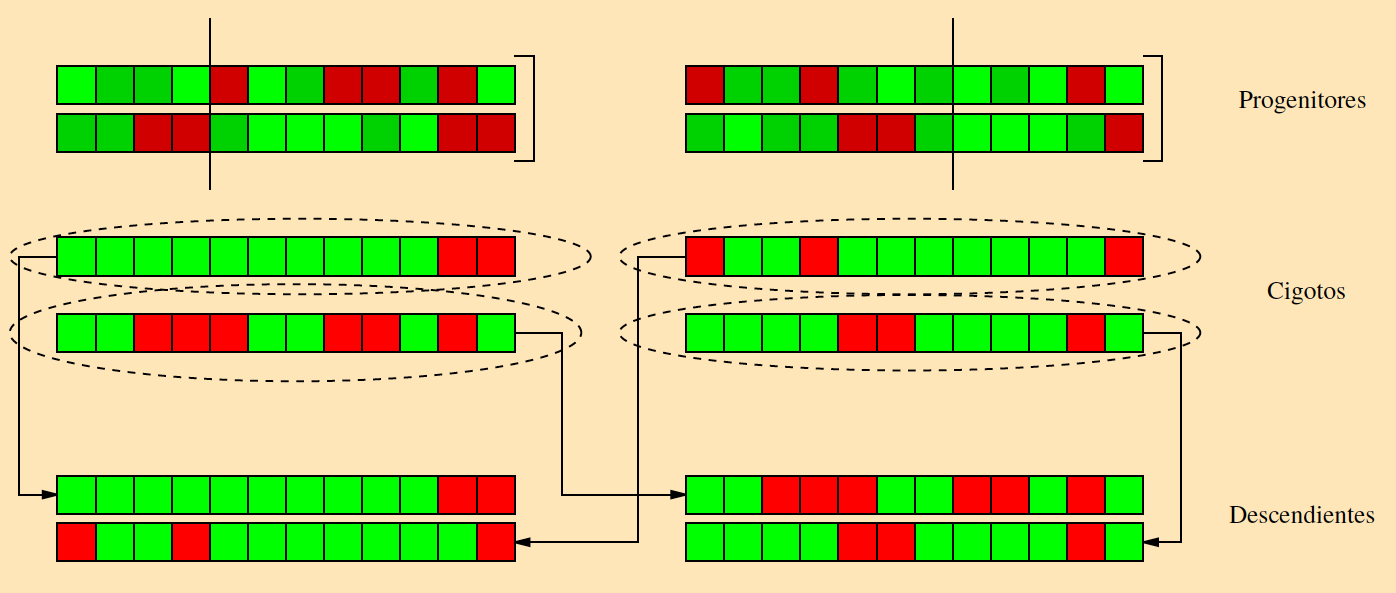
\includegraphics[scale=.4]{reproduccion_diploide.jpg}}
\end{figure}

\subsection{Coevolución}
En lugar de haber un sistema en el entorno hay varios que compiten por los recursos, por lo que los sistemas compiten y tratan de ser superior a otro para sobrevivir.

La coevolución es una fuerza importante hacia la generación de adaptaciones muy complejas.

Relaciones depredador-presa

Existe una gran presión para que las presas se defiendan mejor y en respuesta los depredadores desarrollan mejores estrategias de ataque.

El éxito de una parte es el fracaso de la opuesta que debe desarrollar respuestas para mantener sus posibilidades de supervivencia, el dilema de la Reina roja. Para seguir siendo igual de bueno hay que seguir evolucionando, si no el resto lo harán y nosotros empeoraremos.

Normalmente se habla de 2 sistemas.
\pagebreak

\subsubsection{Coevolución computacional}
\textbf{Tipos:}
\begin{itemize}
	\item \textbf{Cooperativa:} Dos sistemas independientes cooperan para aumentar sus posibilidades de supervivencia
	
	Simbiosis, “vive y deja vivir” en la Primera Guerra Mundial
	\item \textbf{Competitiva:} Dos sistemas independientes compiten por recursos compartidos
	
	Depredador-presa
	
	f1 inversamente proporcional a f2, si S1 mejora S2 tendrá mayor presión para evolucionar.
\end{itemize}

\subsubsection{Evaluación de los individuos}
En algunas ocasiones los individuos de una población tienen que ser evaluados utilizando ejemplos. Hay que generar un conjunto de ejemplos, p. ej. de forma aleatoria, y utilizarlos para evaluar un individuo.

Aparece el problema denominado \textbf{“Ideal trainer”, entrenador ideal}:
\begin{itemize}
	\item Existe un número enorme de posibles ejemplos, pero solo un ínfimo número de ellos se pueden utilizar para evaluar al individuo para que el proceso sea eficiente. El problema está en cómo determinar qué conjunto de n ejemplos (n pequeño) es el “ideal” para que sirva de evaluación. 
	\item Si el conjunto de ejemplos es “fácil” se puede producir especialización. Lo que puede ser un buen conjunto de evaluación para un individuo, puede ser malo para otro y viceversa
\end{itemize}

\subsubsection{Problema del entrenador ideal}
Una primera solución sería generar un \textbf{nuevo conjunto de entrenamiento en cada generación}
\begin{itemize}
	\item Los individuos no podrían especializarse, ya que se evalúan cada vez con ejemplos diferentes.
	\item Un individuo muy bueno en una generación, y que por tanto ha engendrado muchos descendientes, puede ser muy malo en la siguiente, y todos los individuos que ha engendrado ser inoperativos.
	\item Al cambiar bruscamente la evaluación de los individuos el “fitness landscape” se hace muy abrupto, y el método se desorienta.
\end{itemize}

Se podría \textbf{cambiar de conjunto de aprendizaje cada “n” generaciones}. Esto reduciría los problemas anteriores, pero no los eliminaría.

Se podría \textbf{cambiar “ligeramente” el conjunto de aprendizaje cada “n” generaciones}
\begin{itemize}
	\item Habría que ver cuánto y cómo se cambia el conjunto de aprendizaje, y en función de qué.
	\item Al utilizar el mismo conjunto de aprendizaje para todos los individuos, cambios positivos para unos podrían ser negativos para otros.
\end{itemize}

Se podría generar un \textbf{conjunto de aprendizaje diferente para cada individuo, y cambiarlo “ligeramente” cada “n” generaciones}
\begin{itemize}
	\item Se tendría el problema de cuánto y cómo cambiar el conjunto de aprendizaje.
	\item Si el conjunto de aprendizaje es complejo, el problema anterior no es trivial.
\end{itemize}

\subsubsection{Conjuntos de entrenamiento como sistemas genéticos}
La solución es generar una \textbf{población de conjuntos de entrenamiento, cada individuo es un conjunto de entrenamiento}, compuesto por n valores reales.

Cada individuo-conjunto-de-entrenamiento es evaluado con un conjunto de individuos solución.

El resultado de la evaluación se utiliza para evaluar a los individuos-ejemplo y a los individuos-solución, una buena evaluación para un individuo-solución será mala para un individuo-ejemplo y viceversa.

Esta evaluación se utiliza dentro de un Algoritmo Genético, de forma que se evolucionan los conjuntos de entrenamiento más complicados para un individuo-solución o para un conjunto de individuos-solución.

\subsubsection{Life-time fitness}
Dos poblaciones, una de soluciones P$_s$(t) de tamaño $|| P_s ||$ y otra de ejemplos P$_e$ de tamaño $|| P_e ||$.

\textbf{P$_s$(t) evoluciona con el tiempo, P$_e$ se mantiene fija.} Cada individuo de P$_s$ se evalúa sobre los últimos $\tau$ ejemplos, y lo mismo cada individuo de P$_e$.

La evaluación de P$_s$ sirve para seleccionar y generar nuevos individuos, mientras que la de P$_e$ solo para seleccionar individuos. La evaluación es la suma, u otra medida estadística, de encuentros entre soluciones y ejemplos.

\subsubsection{Ciclo coevolutivo}
\begin{enumerate}
	\item Realizar n veces
	\begin{enumerate}
		\item s = seleccionar(P$_s$)
		\item e = seleccionar(P$_e$)
		\item f = encuentro(s, e)
		\item actualizar-fit(s, f) se puede hacer con la media de los fitness
		\item act-fitness(e,1/f) se puede hacer con la media de los fitness
	\end{enumerate}
	\item s$_1$ = seleccionar(P$_s$)
	\item s$_2$ = seleccionar(P$_s$)
	\item s$_{hijo}$ = cruce-mut(s$_1$, s$_2$)
	\item Realizar m veces
	\begin{enumerate}
		\item e = seleccionar(P$_e$)
		\item f = encuentro(s$_{hijo}$, e)
		\item f(s$_{hijo}$) = actualizar-fit(s$_{hijo}$, f)
		\item f(e) = actualizar-fit(e,1/f)
	\end{enumerate}
	\item insertar(s$_{hijo}$, f(s$_{hijo}$), P$_s$)
\end{enumerate}

\textbf{Funciones}
\begin{itemize}
	\item \textbf{Seleccionar(P)}. selecciona un elemento de la población (P), de manera proporcional a su fitness.
	\item \textbf{Actualizar fitness(i, f)}. Cada individuo (i) lleva una memoria del resultado de los últimos m encuentros, al actualizar, se elimina de la memoria el resultado del encuentro más antiguo, se añade el actual (f), y se recalcula su fitness.
	\item \textbf{Encuentro(s, e)}. La solución s se evalúa con el ejemplo e y obtenemos un valor de fitness para este encuentro.
	\item \textbf{Insertar(s, f(s), P)}. Si f(s) es mejor que el fitness del peor individuo de la población.
\end{itemize}

\textbf{Características}
\begin{itemize}
	\item Las soluciones solo se evalúan con un conjunto pequeño (m) de ejemplos, en vez de con todos los posibles.
	\item Al principio todos los ejemplos tienen la misma probabilidad de ser seleccionados, pero a medida que son evaluados unos tienen más probabilidad que otros.
	\item Los \textbf{ejemplos más difíciles tendrán mejor fitness y mayor probabilidad de ser elegidos}.
	\item Al utilizar una ventana temporal de m para el cálculo del fitness, tanto soluciones como ejemplos se adaptarán unos a otros.
\end{itemize}

\end{document}